\subsection{Eletrônica}

Como um dos maiores problemas do MVP foi o de falha no sistema eletrônico devido a mal-contato, atenção especial foi dada a esta parte. Duas soluções foram propostas:

\begin{itemize}
    \item Produção de placas de circuito impresso para todos os sistemas
    \item Utilização de conectores mais robustos
\end{itemize}

Foram projetadas e produzidas duas PCBs: uma para os transdutores de célula de carga e outra para os transdutores de pressão diferencial, mostradas nas figuras \ref{projeto_pcb_pitot} e \ref{projeto_pcb_celulas}.

\begin{figure}[!ht]
    \centering
    \caption{Projeto e execução da placa de transdutores de pressão diferencial. Fonte: O autor.}
        \subfloat[Projeto da placa no software Autodesk Eagle.]{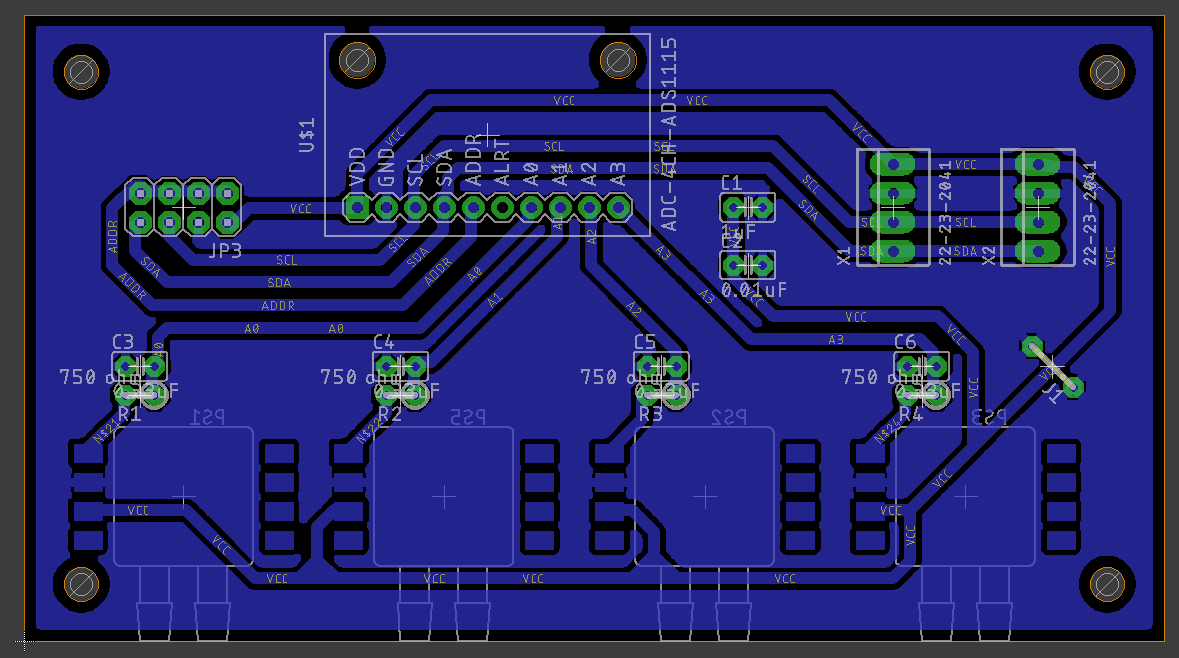
\includegraphics[width=0.4\columnwidth]{figuras/renders/pitot_board.png}}
        \label{projeto_pcb_pitot}
        \qquad
        \subfloat[Placa fresada e com sensores instalados.]{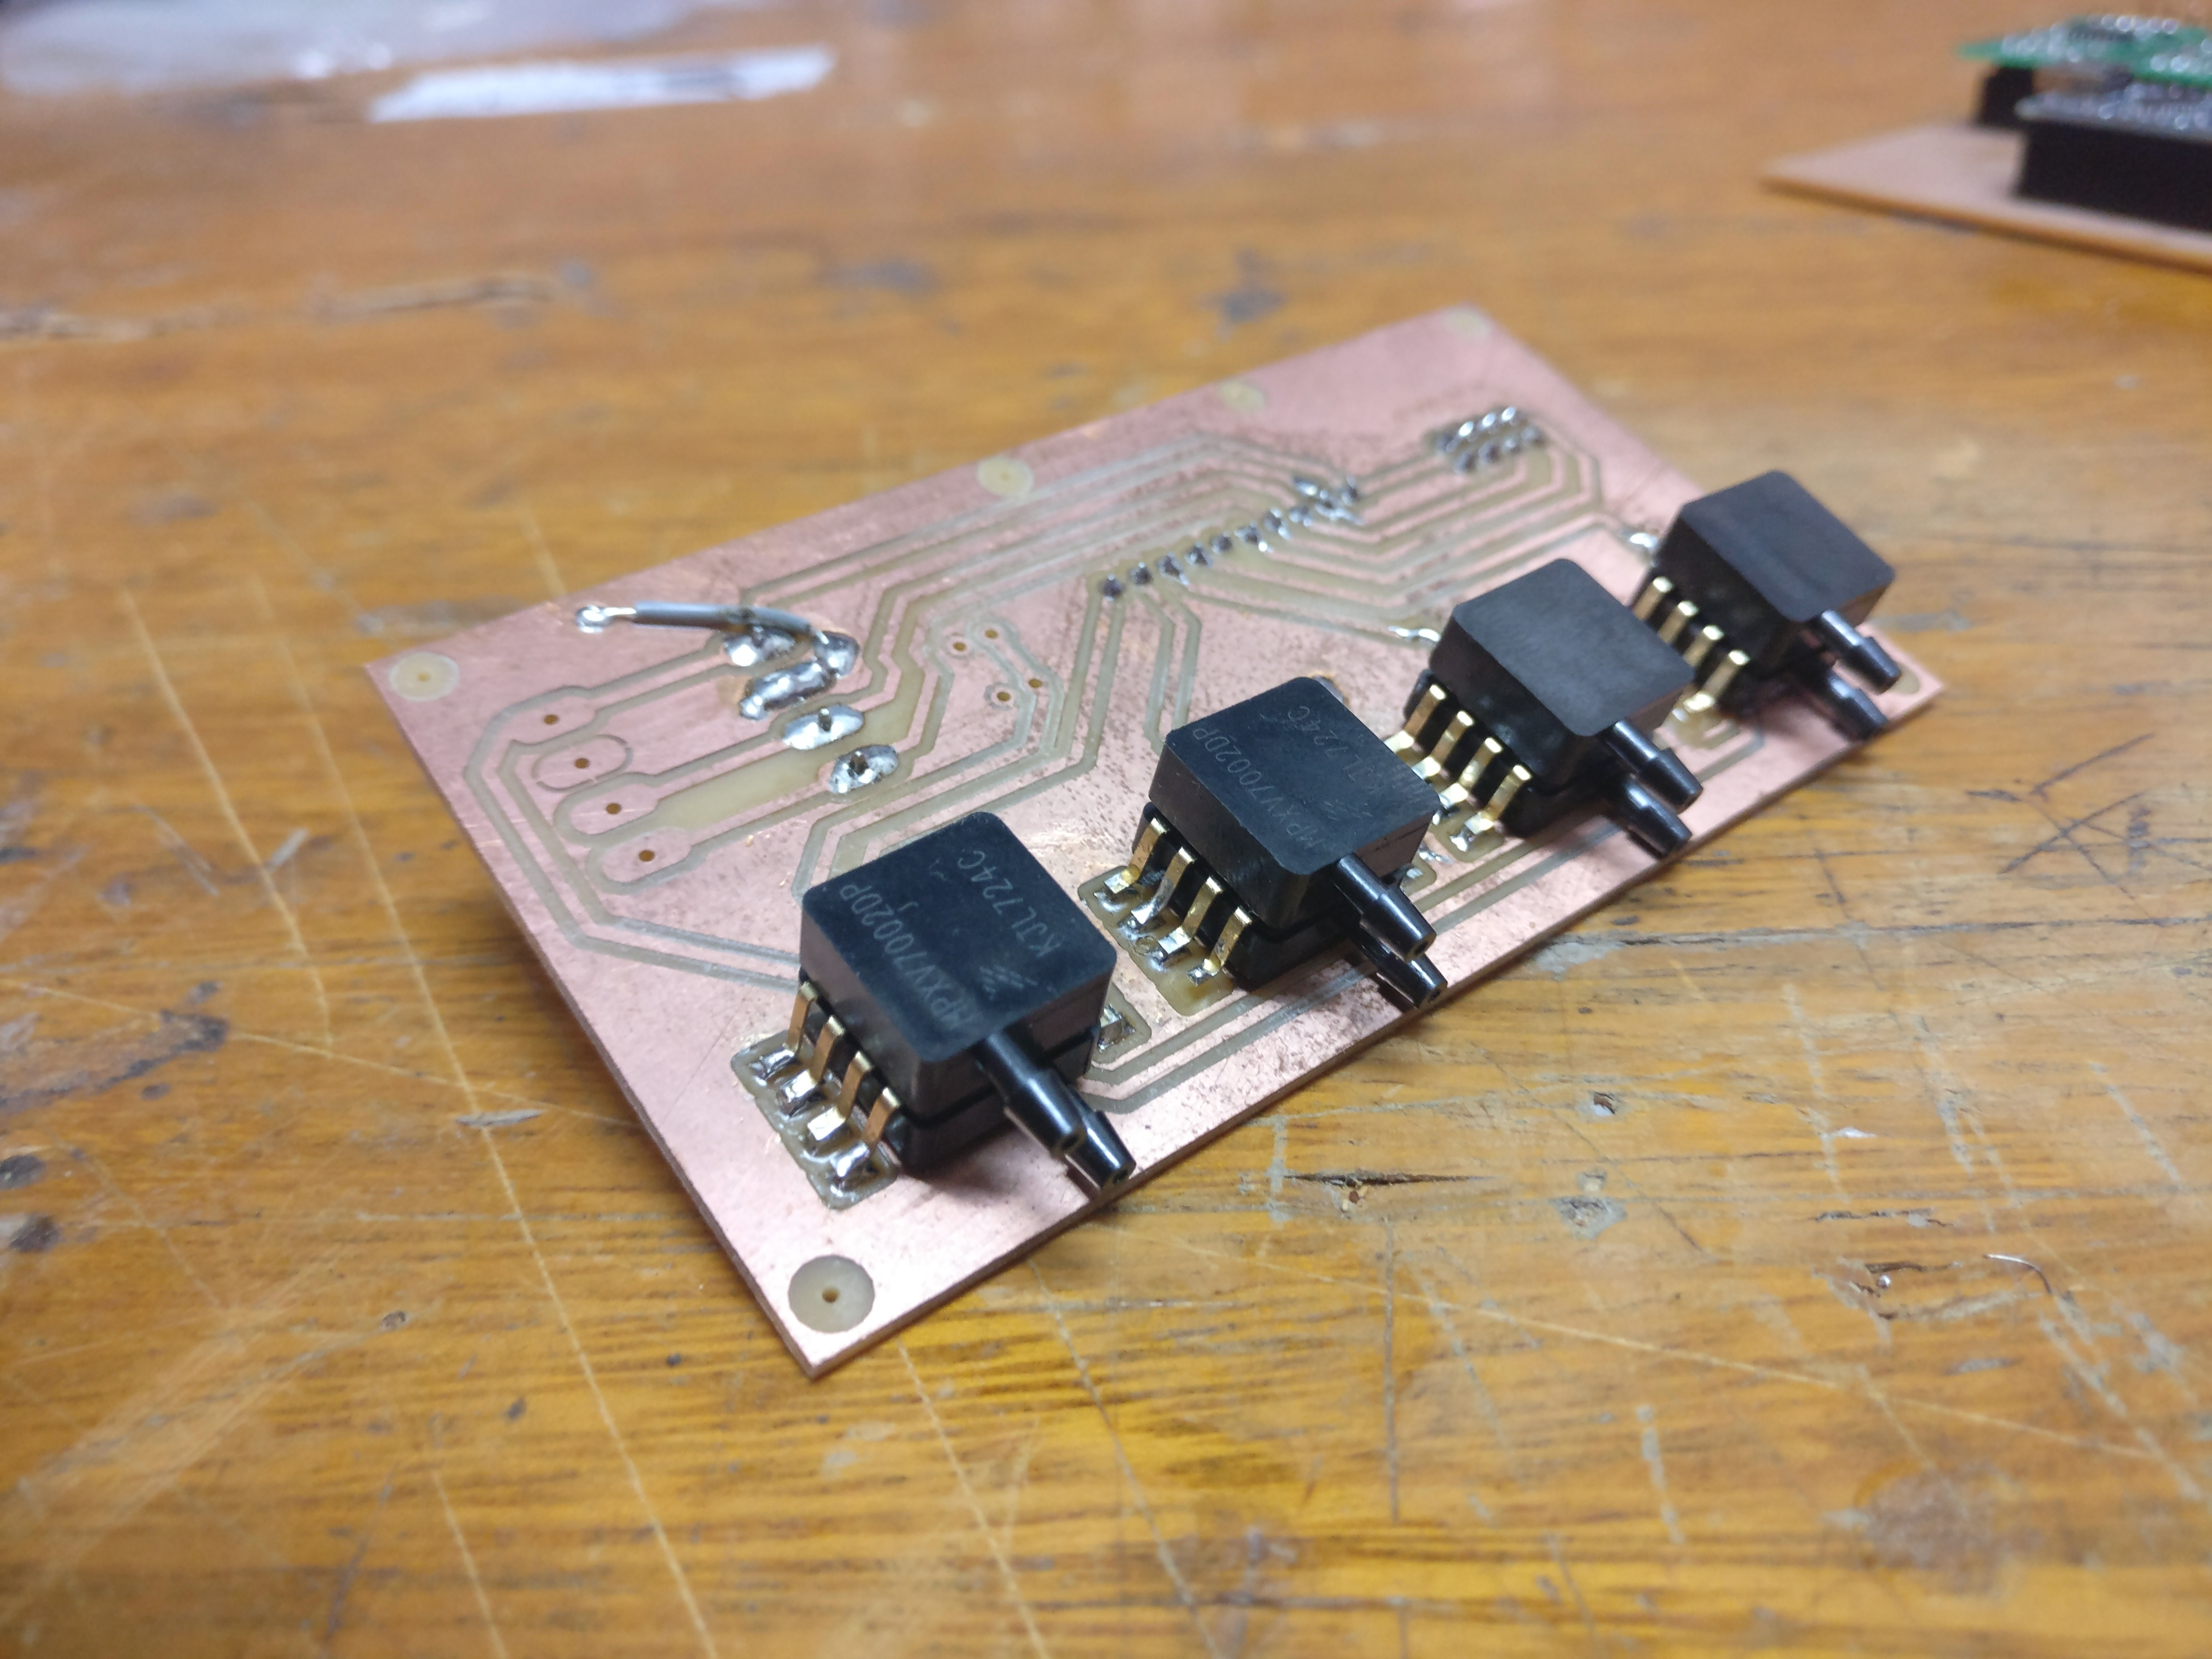
\includegraphics[width=0.4\columnwidth]{figuras/construcao/pcbs_montadas_2.jpg}}
        \label{placa_pcb_pitot}
\end{figure}

\begin{figure}[!ht]
    \centering
    \caption{Projeto e execução da placa de transdutores de pressão diferencial. Fonte: O autor.}
        \subfloat[Projeto da placa no software Autodesk Eagle.]{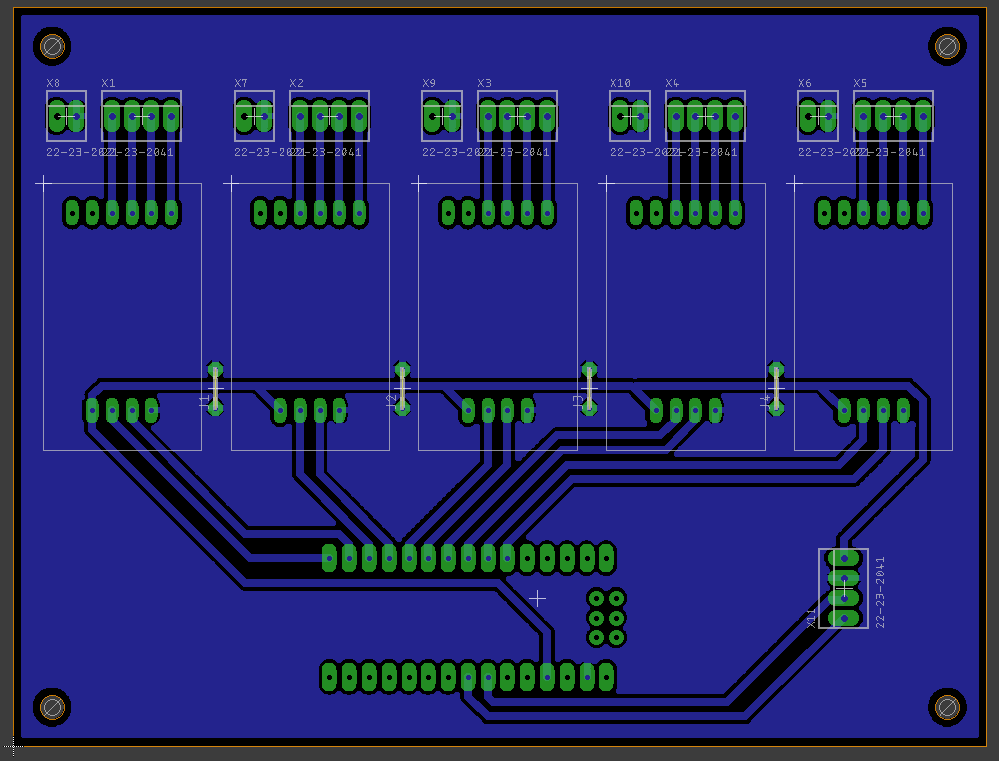
\includegraphics[width=0.4\columnwidth]{figuras/renders/loadcell_board.png}}
        \label{projeto_pcb_celulas}
        \qquad
        \subfloat[Placa fresada e com sensores instalados.]{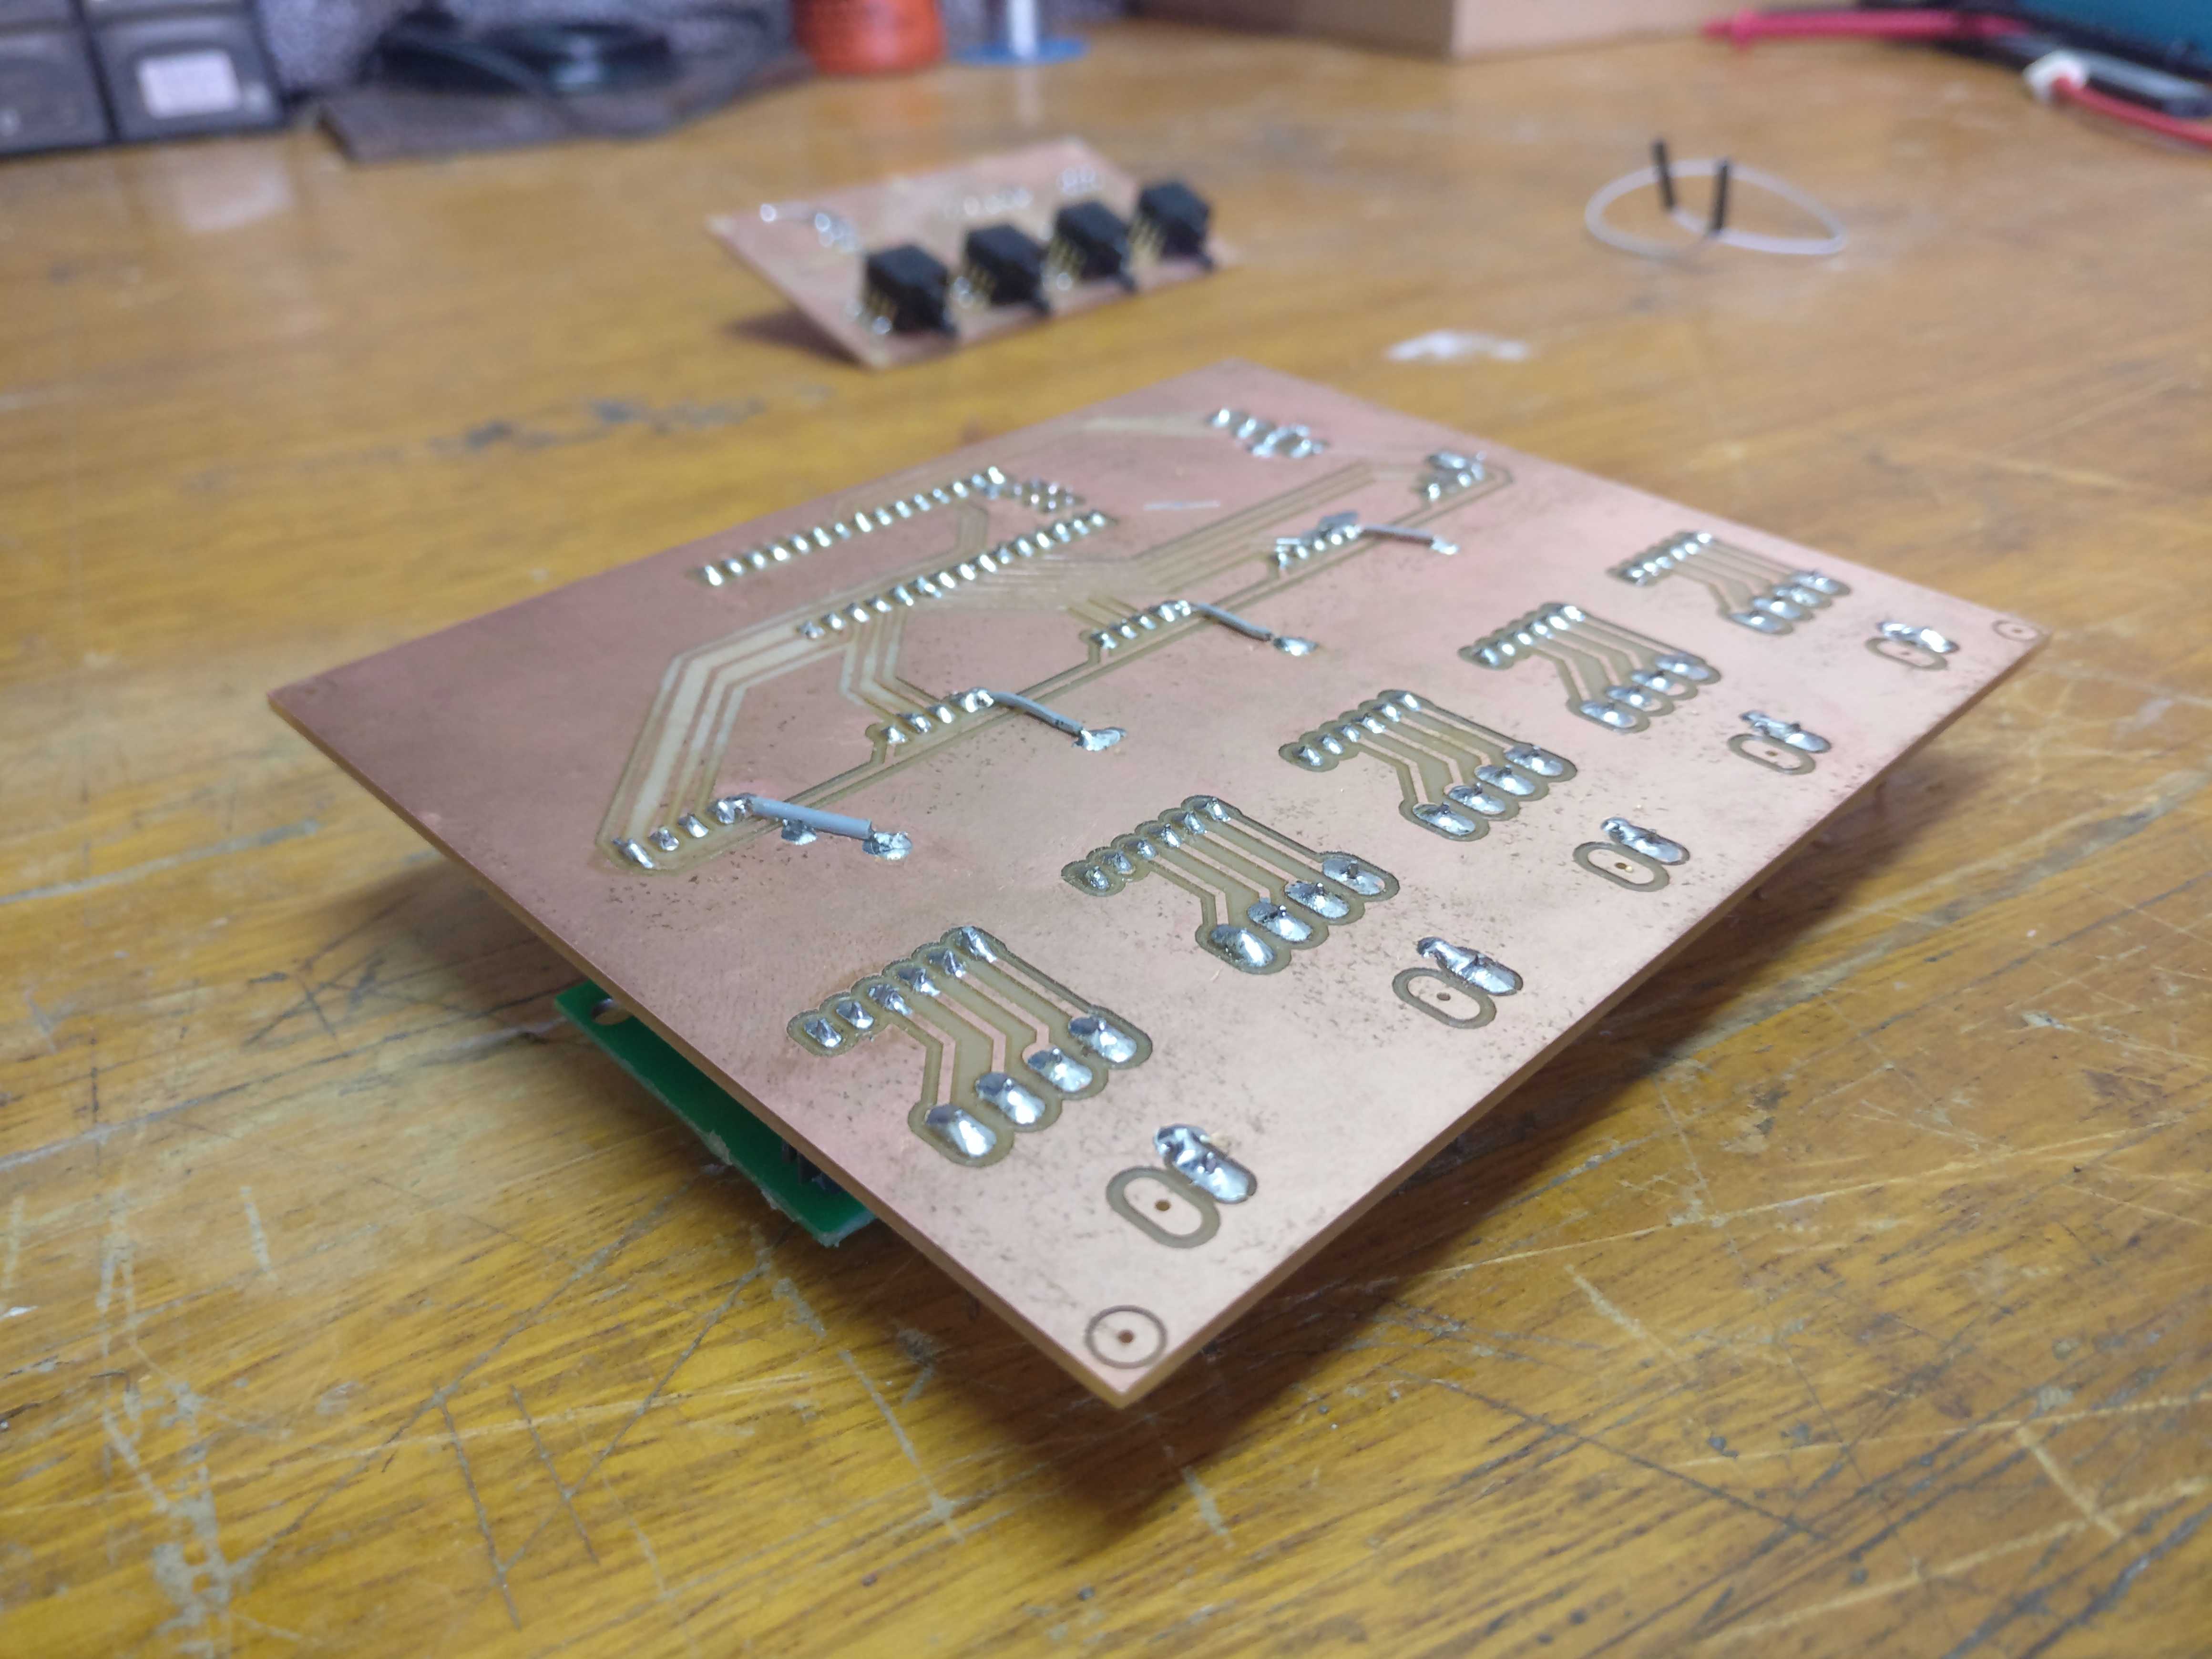
\includegraphics[width=0.4\columnwidth]{figuras/construcao/pcbs_montadas_3.jpg}}
        \label{placa_pcb_celulas}
\end{figure}

Foram confeccionados carcaças para alocação de ambas as placas e seus conectores. Os conectores usados neste projeto foram do modelo GX16, popularmente conhecidos como "conectores de aviação". Estes possuem trava rosqueada e ótimo contato elétrico. Os conectores ficam presos no case e não na placa, de modo que em caso de acidentes de tracionamento dos cabos as placas não sejam danificadas. As versões finais das placas, já instaladas em seus respectivos cases são mostradas nas figuras \ref{case_pitot}a e \ref{case_celulas}b.

\begin{figure}[!ht]
    \centering
    \caption{Cases desenvolvidos para as placas de aquisição. Fonte: O autor.}
        \subfloat[Hardware para aquisição dos dados de velocidade e ângulo de ataque do escoamento.]{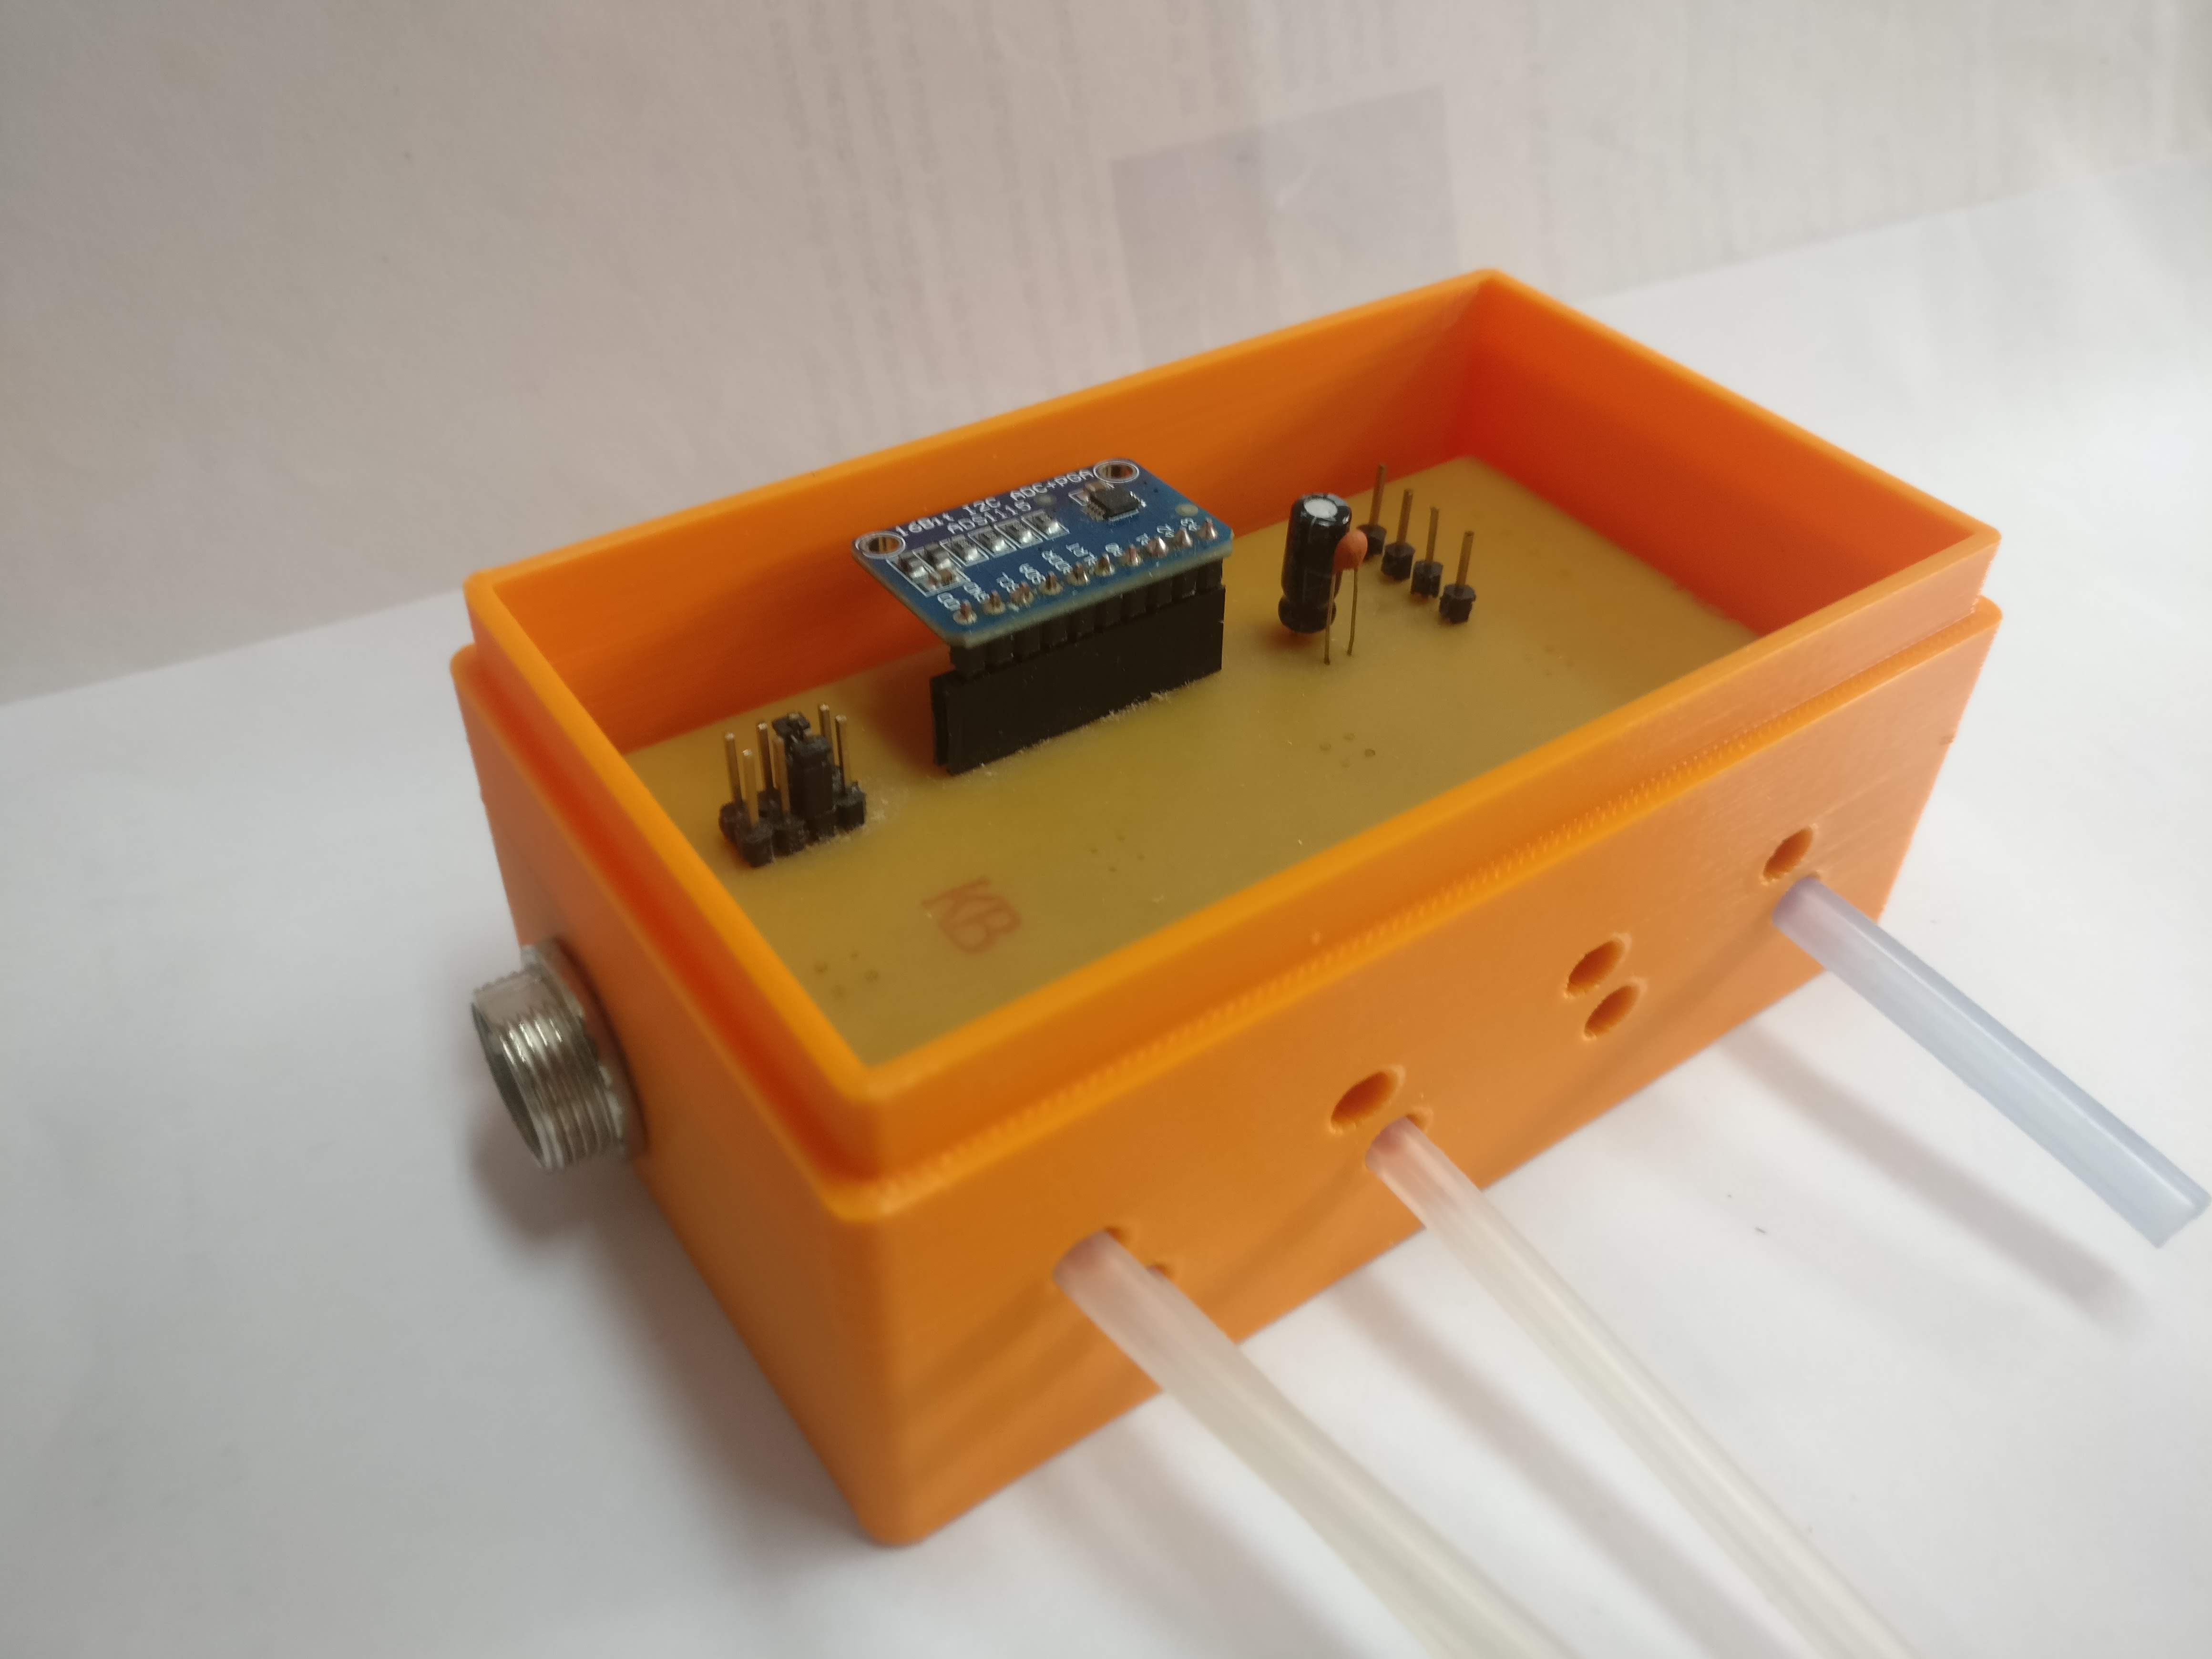
\includegraphics[width=0.4\columnwidth]{figuras/calibracao/caixa_pitot.jpg}}
        \label{case_pitot}
        \qquad
        \subfloat[Hardware para aquisição das cargas aerodinâmicas.]{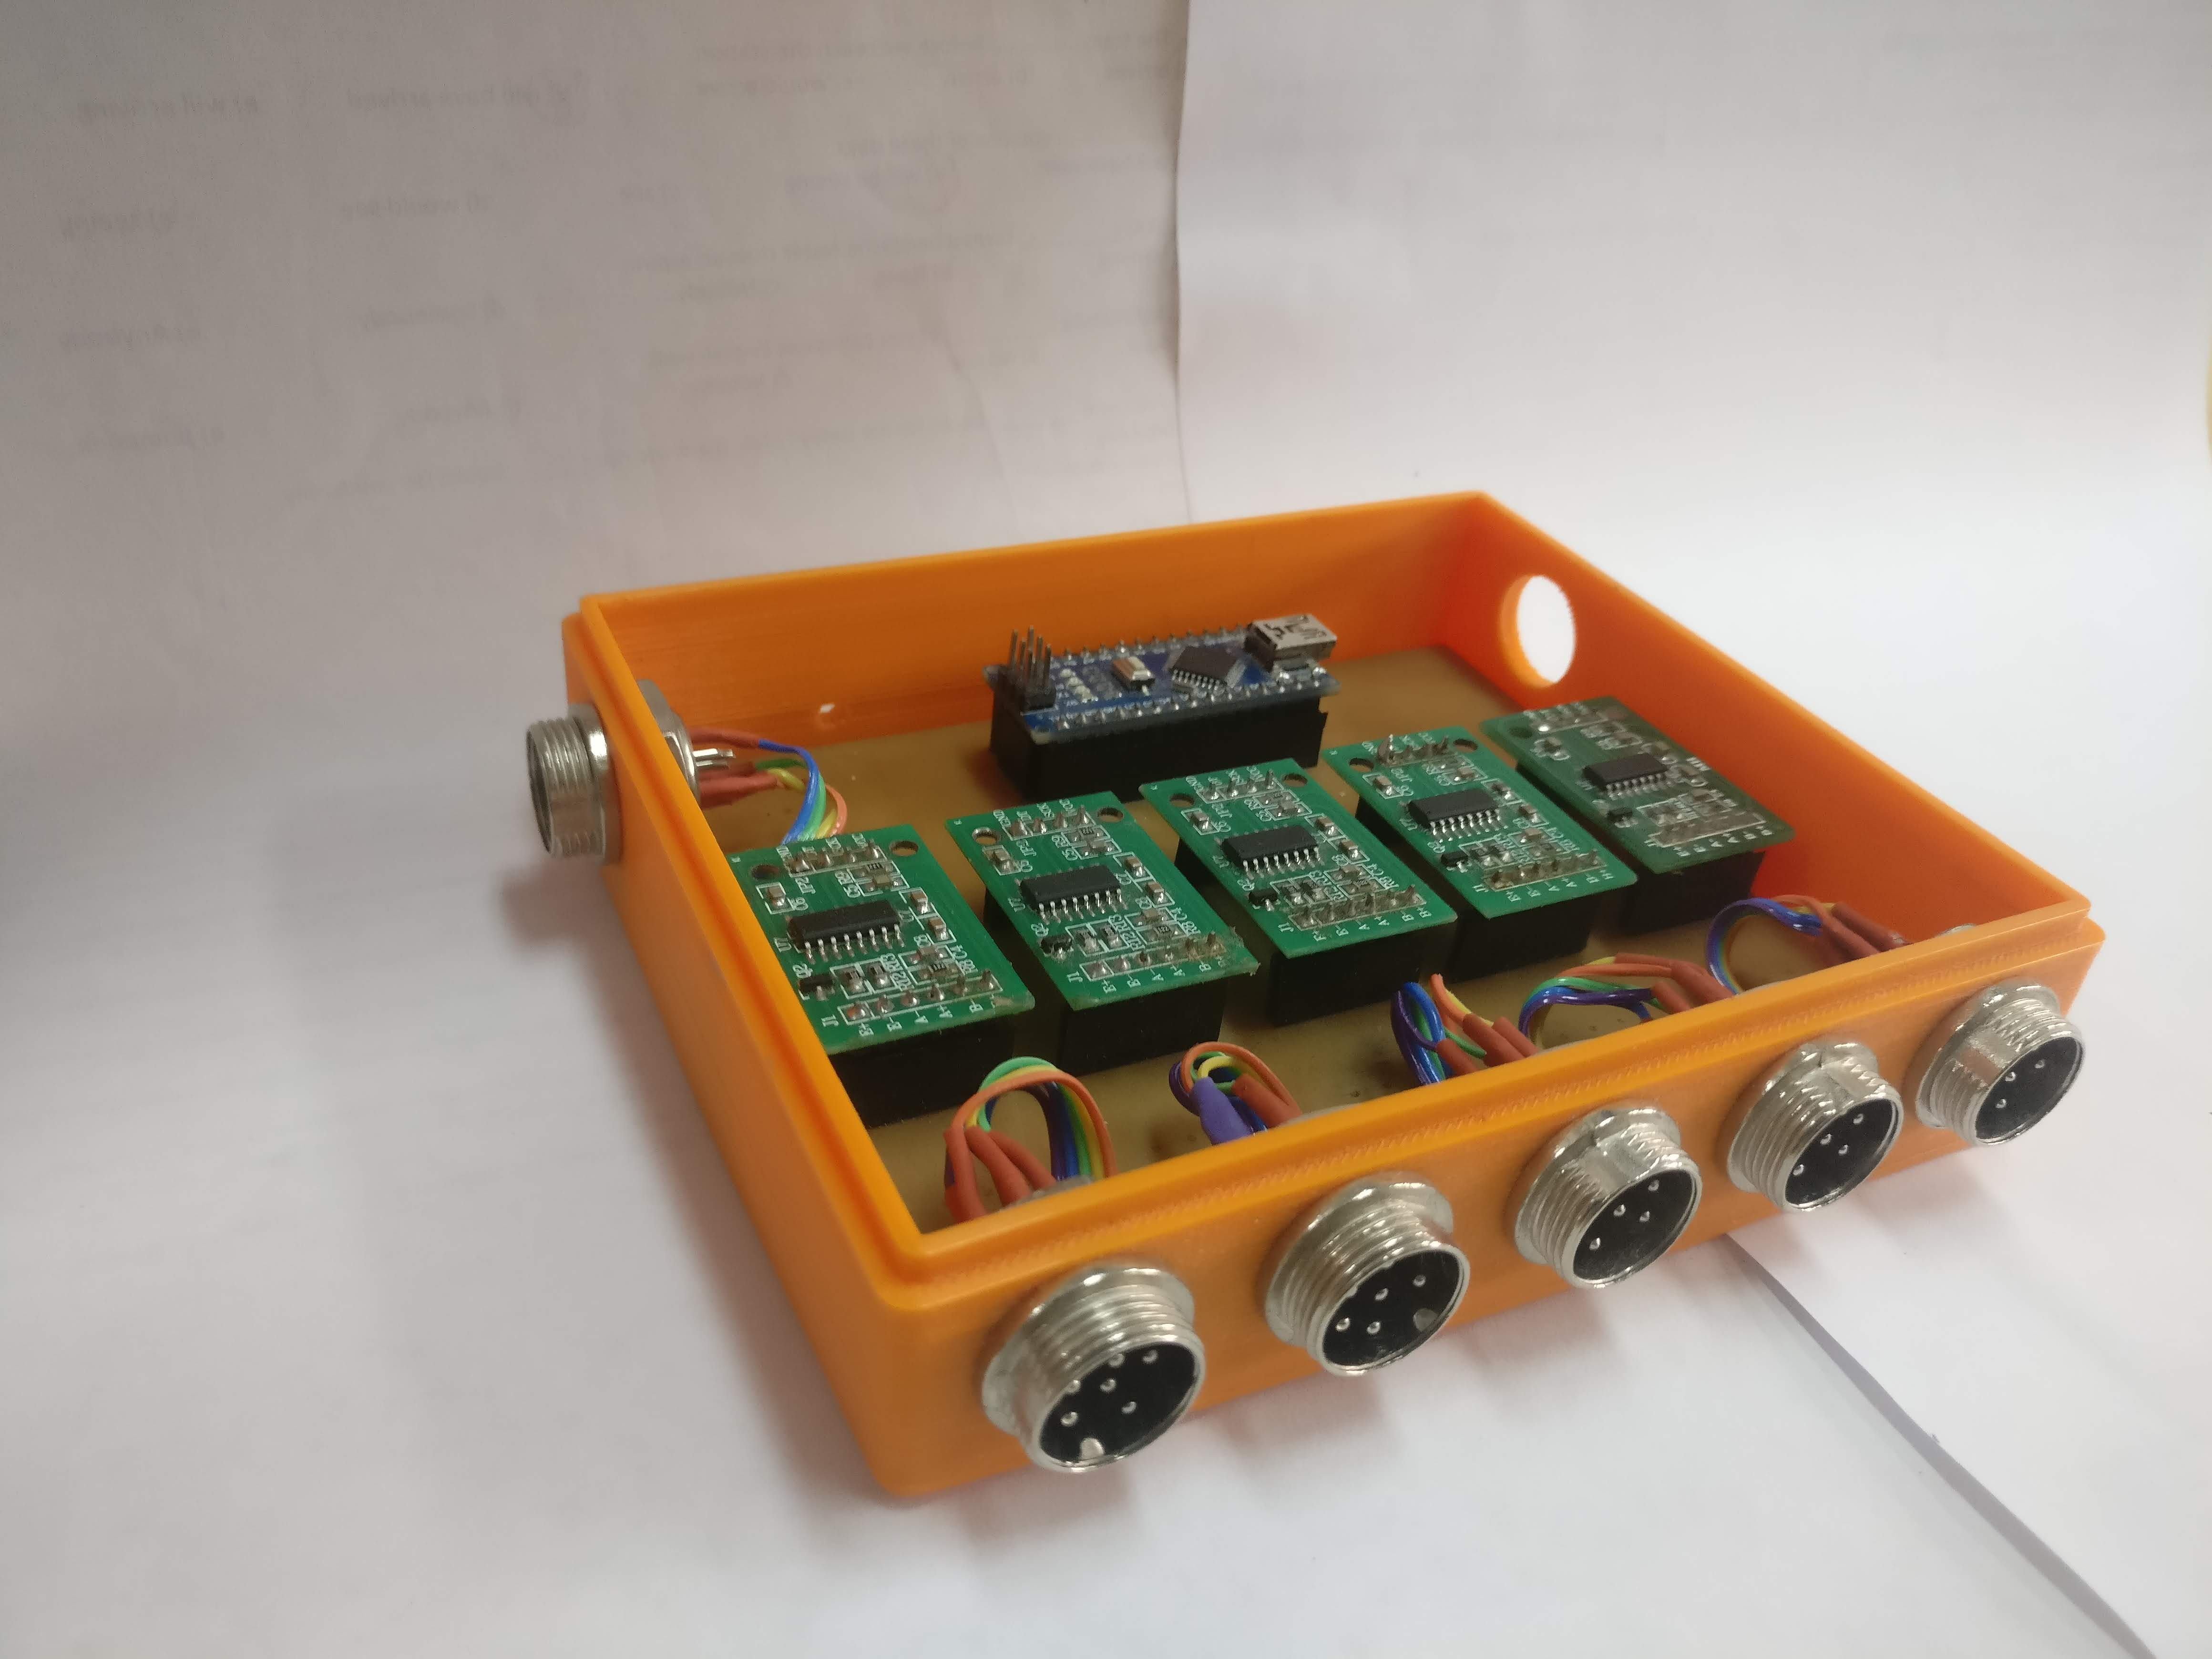
\includegraphics[width=0.4\columnwidth]{figuras/calibracao/caixa_celulas.jpg}}
        \label{case_celulas}
\end{figure}

\subsection{Software Embarcado}

Como já mencionado, todo o software embarcado foi refatorado da versão MVP para esta primeira versão final. Alguns pontos principais merecem destaque:

\begin{itemize}
    \item Integração do Arduino como sensor na plataforma central, permitindo que mais Arduinos sejam conectados paralelamente de forma simplificada
    \item Implementação de nova rotina de ligação da bancada, adaptando automaticamente as configurações internas aos sensores que estiverem conectados, evitando a necessidade de alterar o código toda vez que um novo teste for executado
    \item Implementação de rotina de configuração do teste remotamente via app, permitindo que o operador inclua no arquivo de dados detalhes do teste como o dispositivo testado, seu ângulo de incidência e outras condições, facilitando o entendimento dos dados pelo responsável por processa-los 
    \item Inclusão de código para uso da sonda de ângulo de ataque através dos sensores de pressão diferencial
    \item Transferência de todas as configurações do software para um arquivo de configuração simplificada, permitindo que pessoas sem experiencia com o software embarcado consigam realizar configurações avançadas de forma simples
\end{itemize}

Sobre o primeiro ponto, na versão MVP o Arduino que fazia a aquisição do sinal das células não se comunicava com o Raspberry Pi (plataforma central). Deste modo, seus dados não possuíam sincronia, e esta deveria ser feita posteriormente por quem fosse se utilizar dos dados. Além de exigir um grande trabalho manual, este processo muitas vezes não ficava com qualidade satisfatória, e os dados acabavam não sincronizados. Para resolver este problema o Arduino passou a ser conectado na plataforma central e tratado por esta como um sensor, que responde a pedidos de envio de dados. Para garantir robustez na troca de dados foi implementado protocolo de comunicação de dois sentidos com confirmação de recebimento e checksum (valor calculado nos dois sistemas de forma independente, com base nos demais dados comunicados, de forma a validá-los).

\subsection{Bancada final}

As figuras \ref{fig:render_bancada_completa} e \ref{fig:bancada_construida} mostram a modelagem final da bancada e mesma construída.

\begin{figure}[!ht]
    \centering
    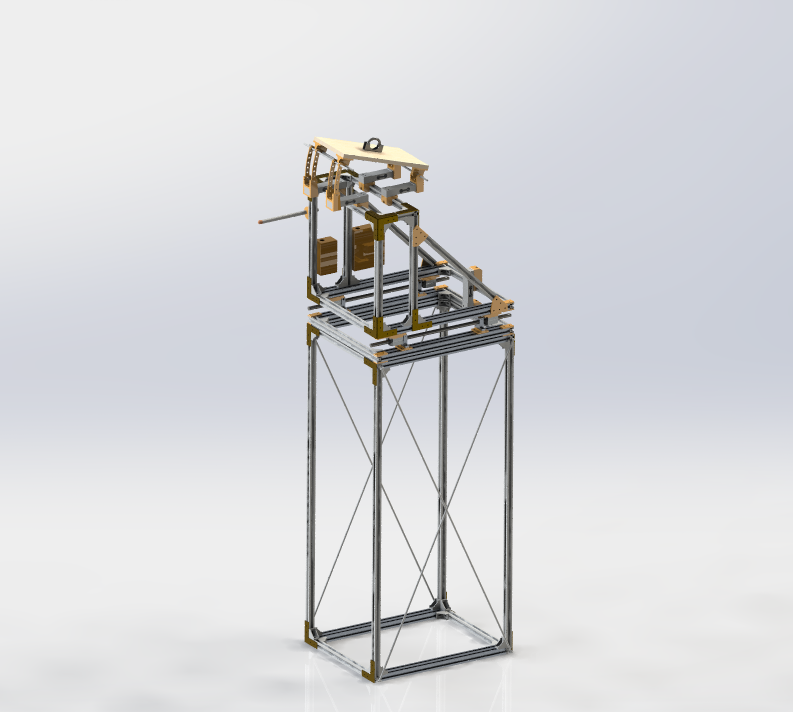
\includegraphics[width=.8\linewidth]{figuras/renders/perspectiva_sem_asa_com_pitot.png}
    \caption{Renderização da bancada modelada no software Solidworks 2016. Fonte: O autor.}
    \label{fig:render_bancada_completa}
\end{figure}

\begin{figure}[!ht]
    \centering
    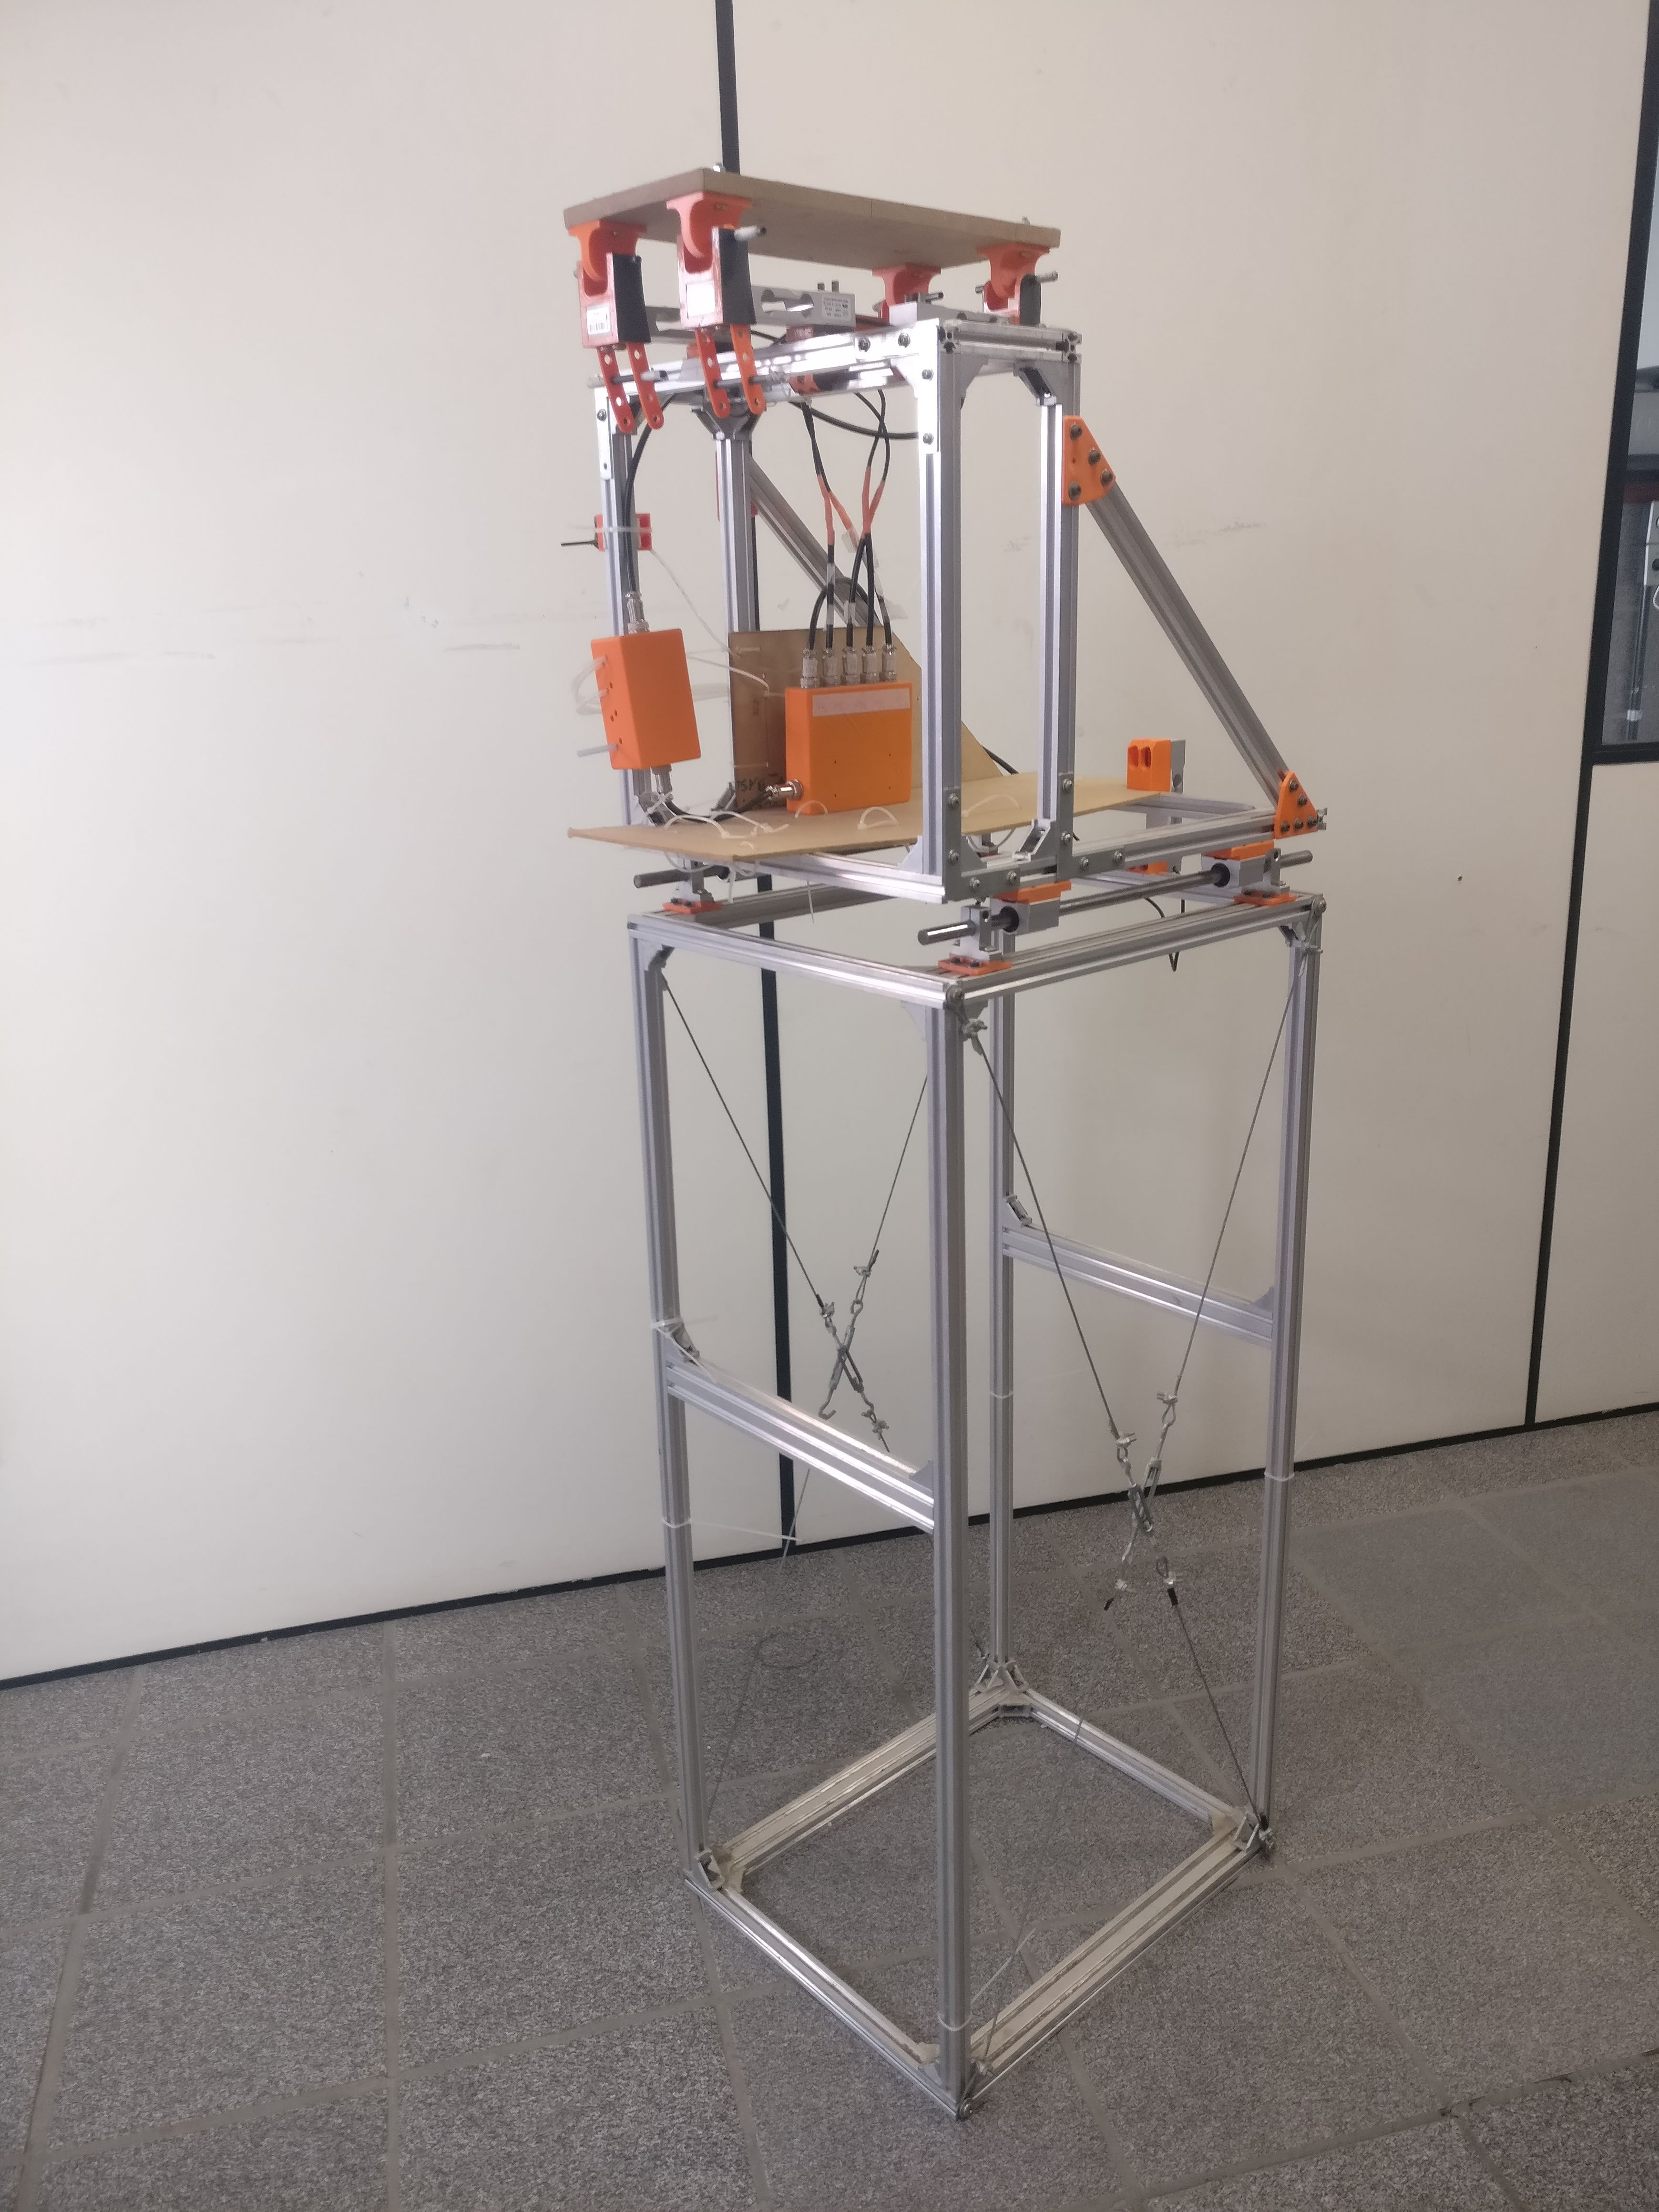
\includegraphics[width=.8\linewidth]{figuras/calibracao/bancada_completa.jpg}
    \caption{Foto da bancada construída. Fonte: O autor.}
    \label{fig:bancada_construida}
\end{figure}

\section{Calibração}

\subsection{Calibração individual das células}
A calibração individual das células foi primeiramente realizada utilizando-se um sistemas de cordas e polias com pesos nas pontas (figuras \ref{polias_1}a e \ref{polias_1}b).

\begin{figure}[!ht]
    \centering
    \caption{Sistema de pesos e polias utilizado inicialmente para calibração das células. Fonte: O autor.}
        \subfloat[Polia utilizada para carregamento vertical.]{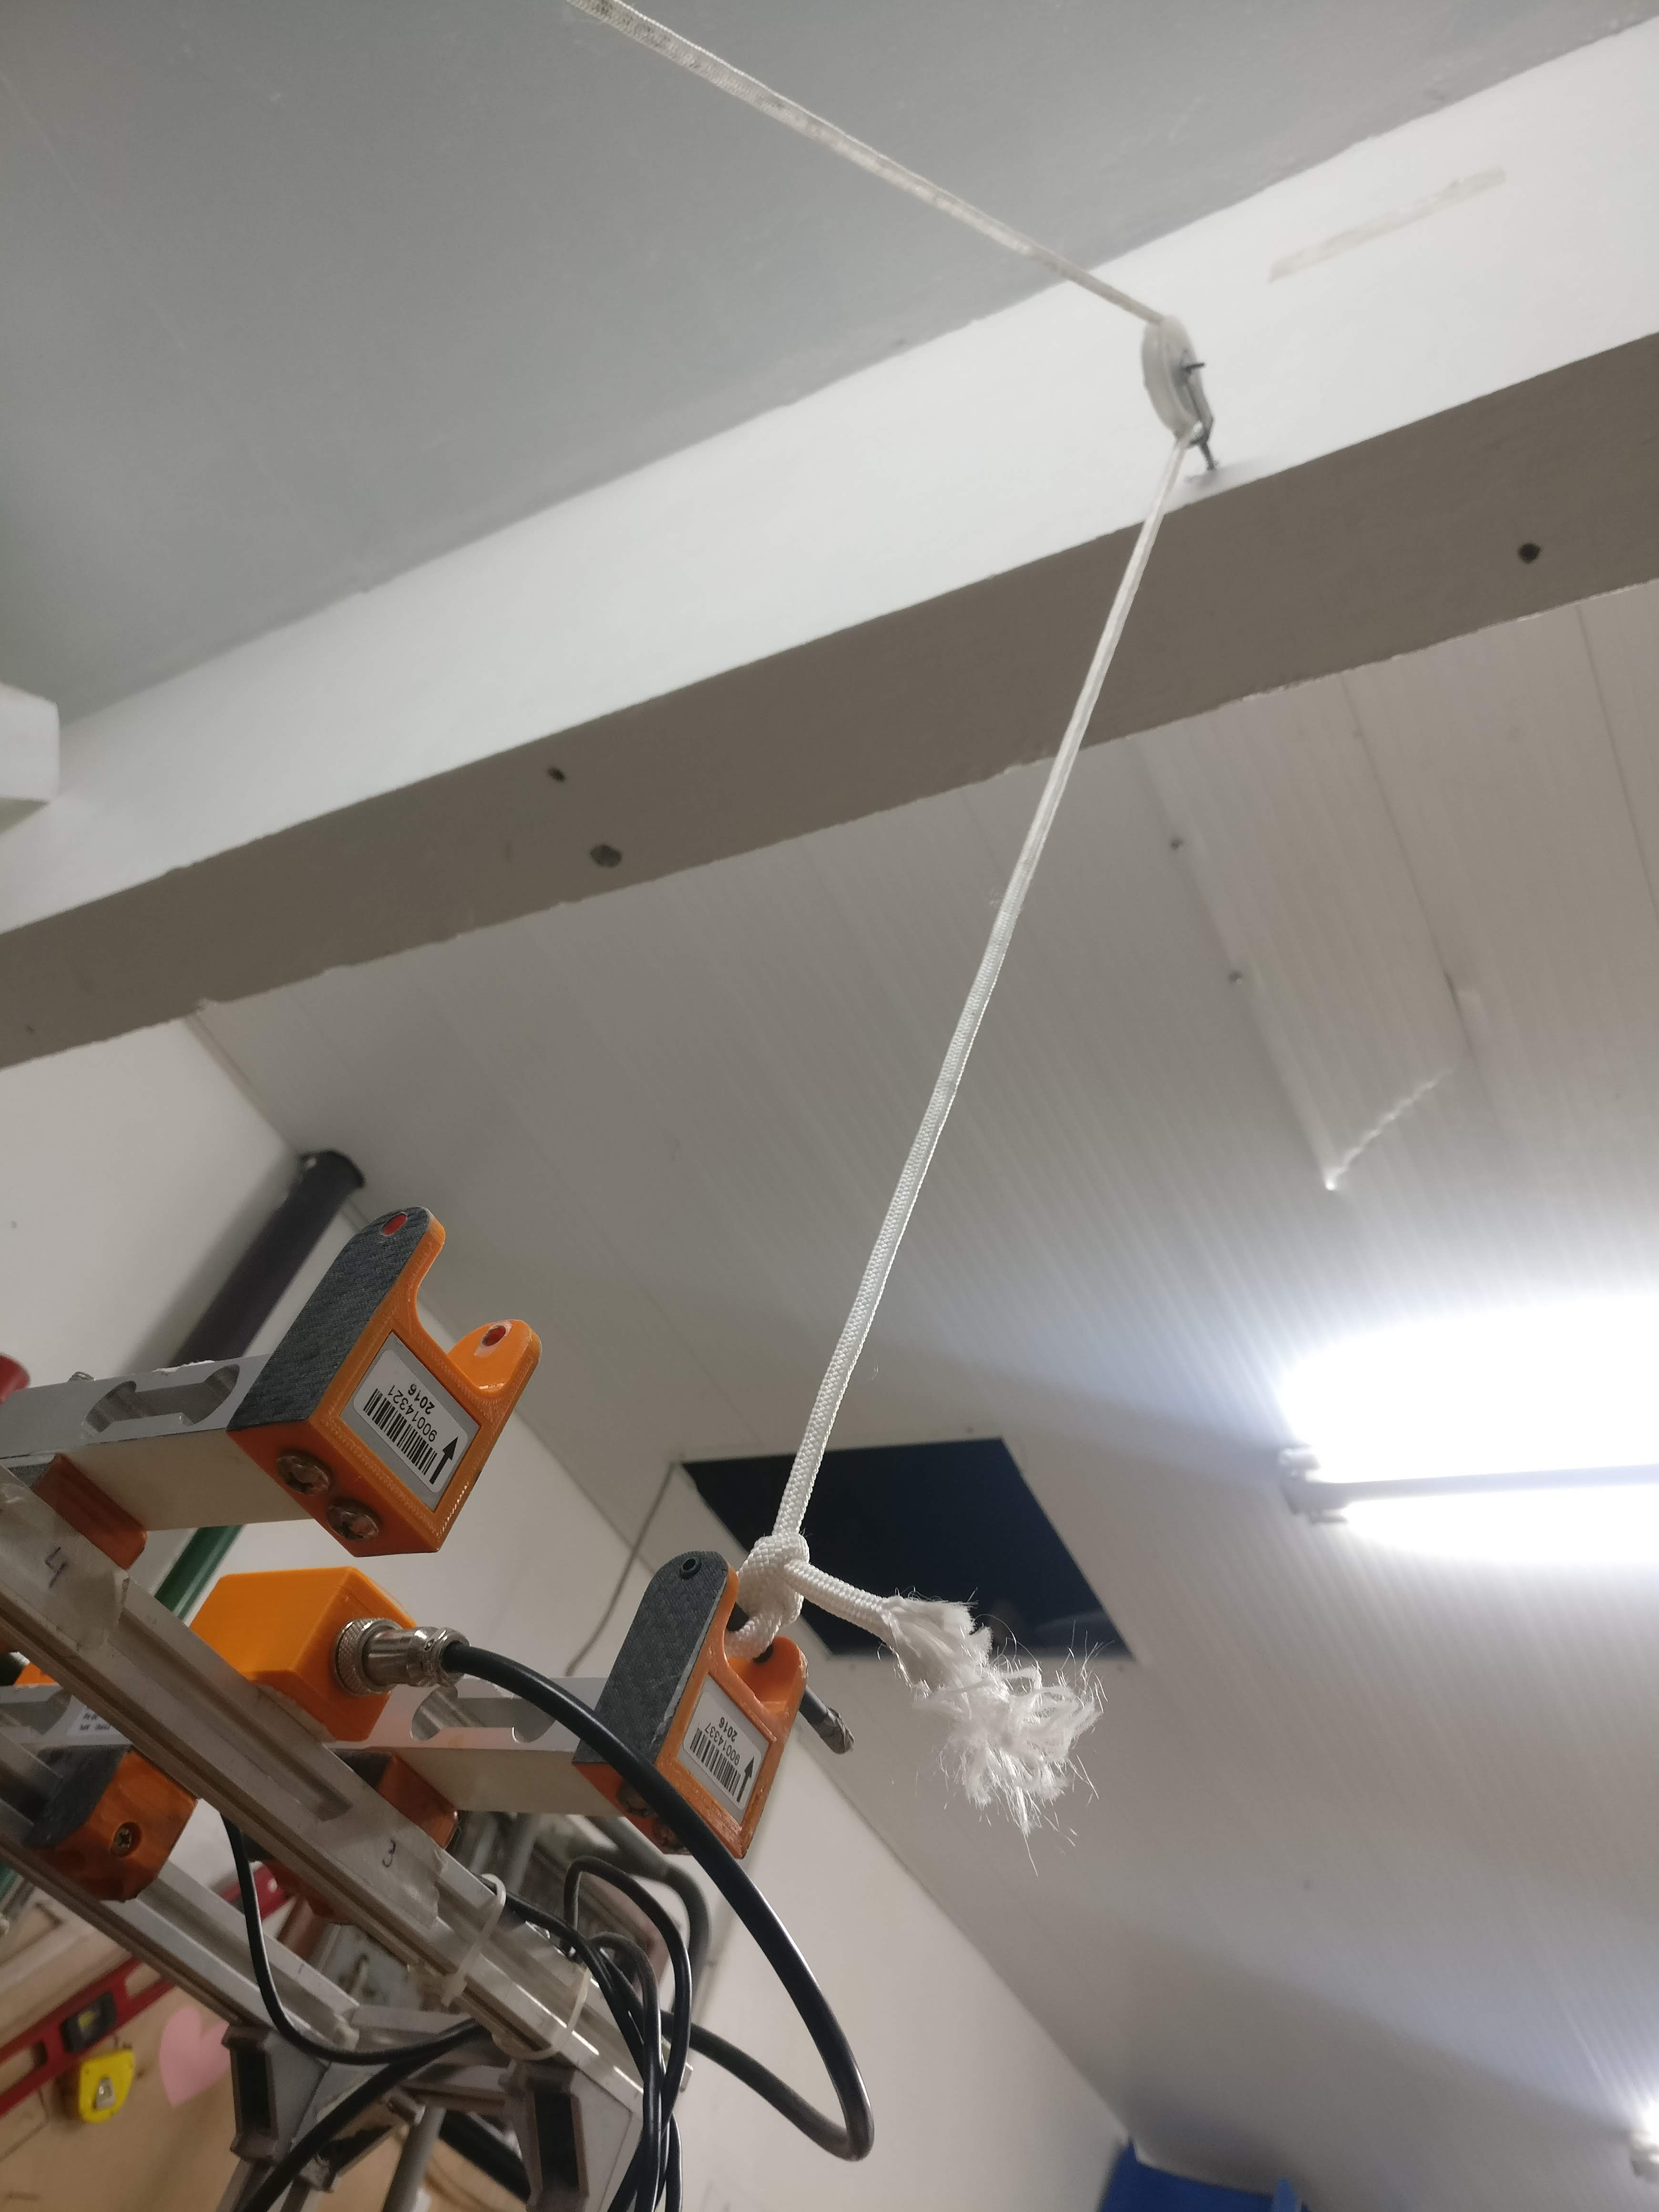
\includegraphics[width=0.4\columnwidth]{figuras/calibracao/polia1.jpg}}
        \label{polias_1}
        \qquad
        \subfloat[Peso utilizado para carregamento das células.]{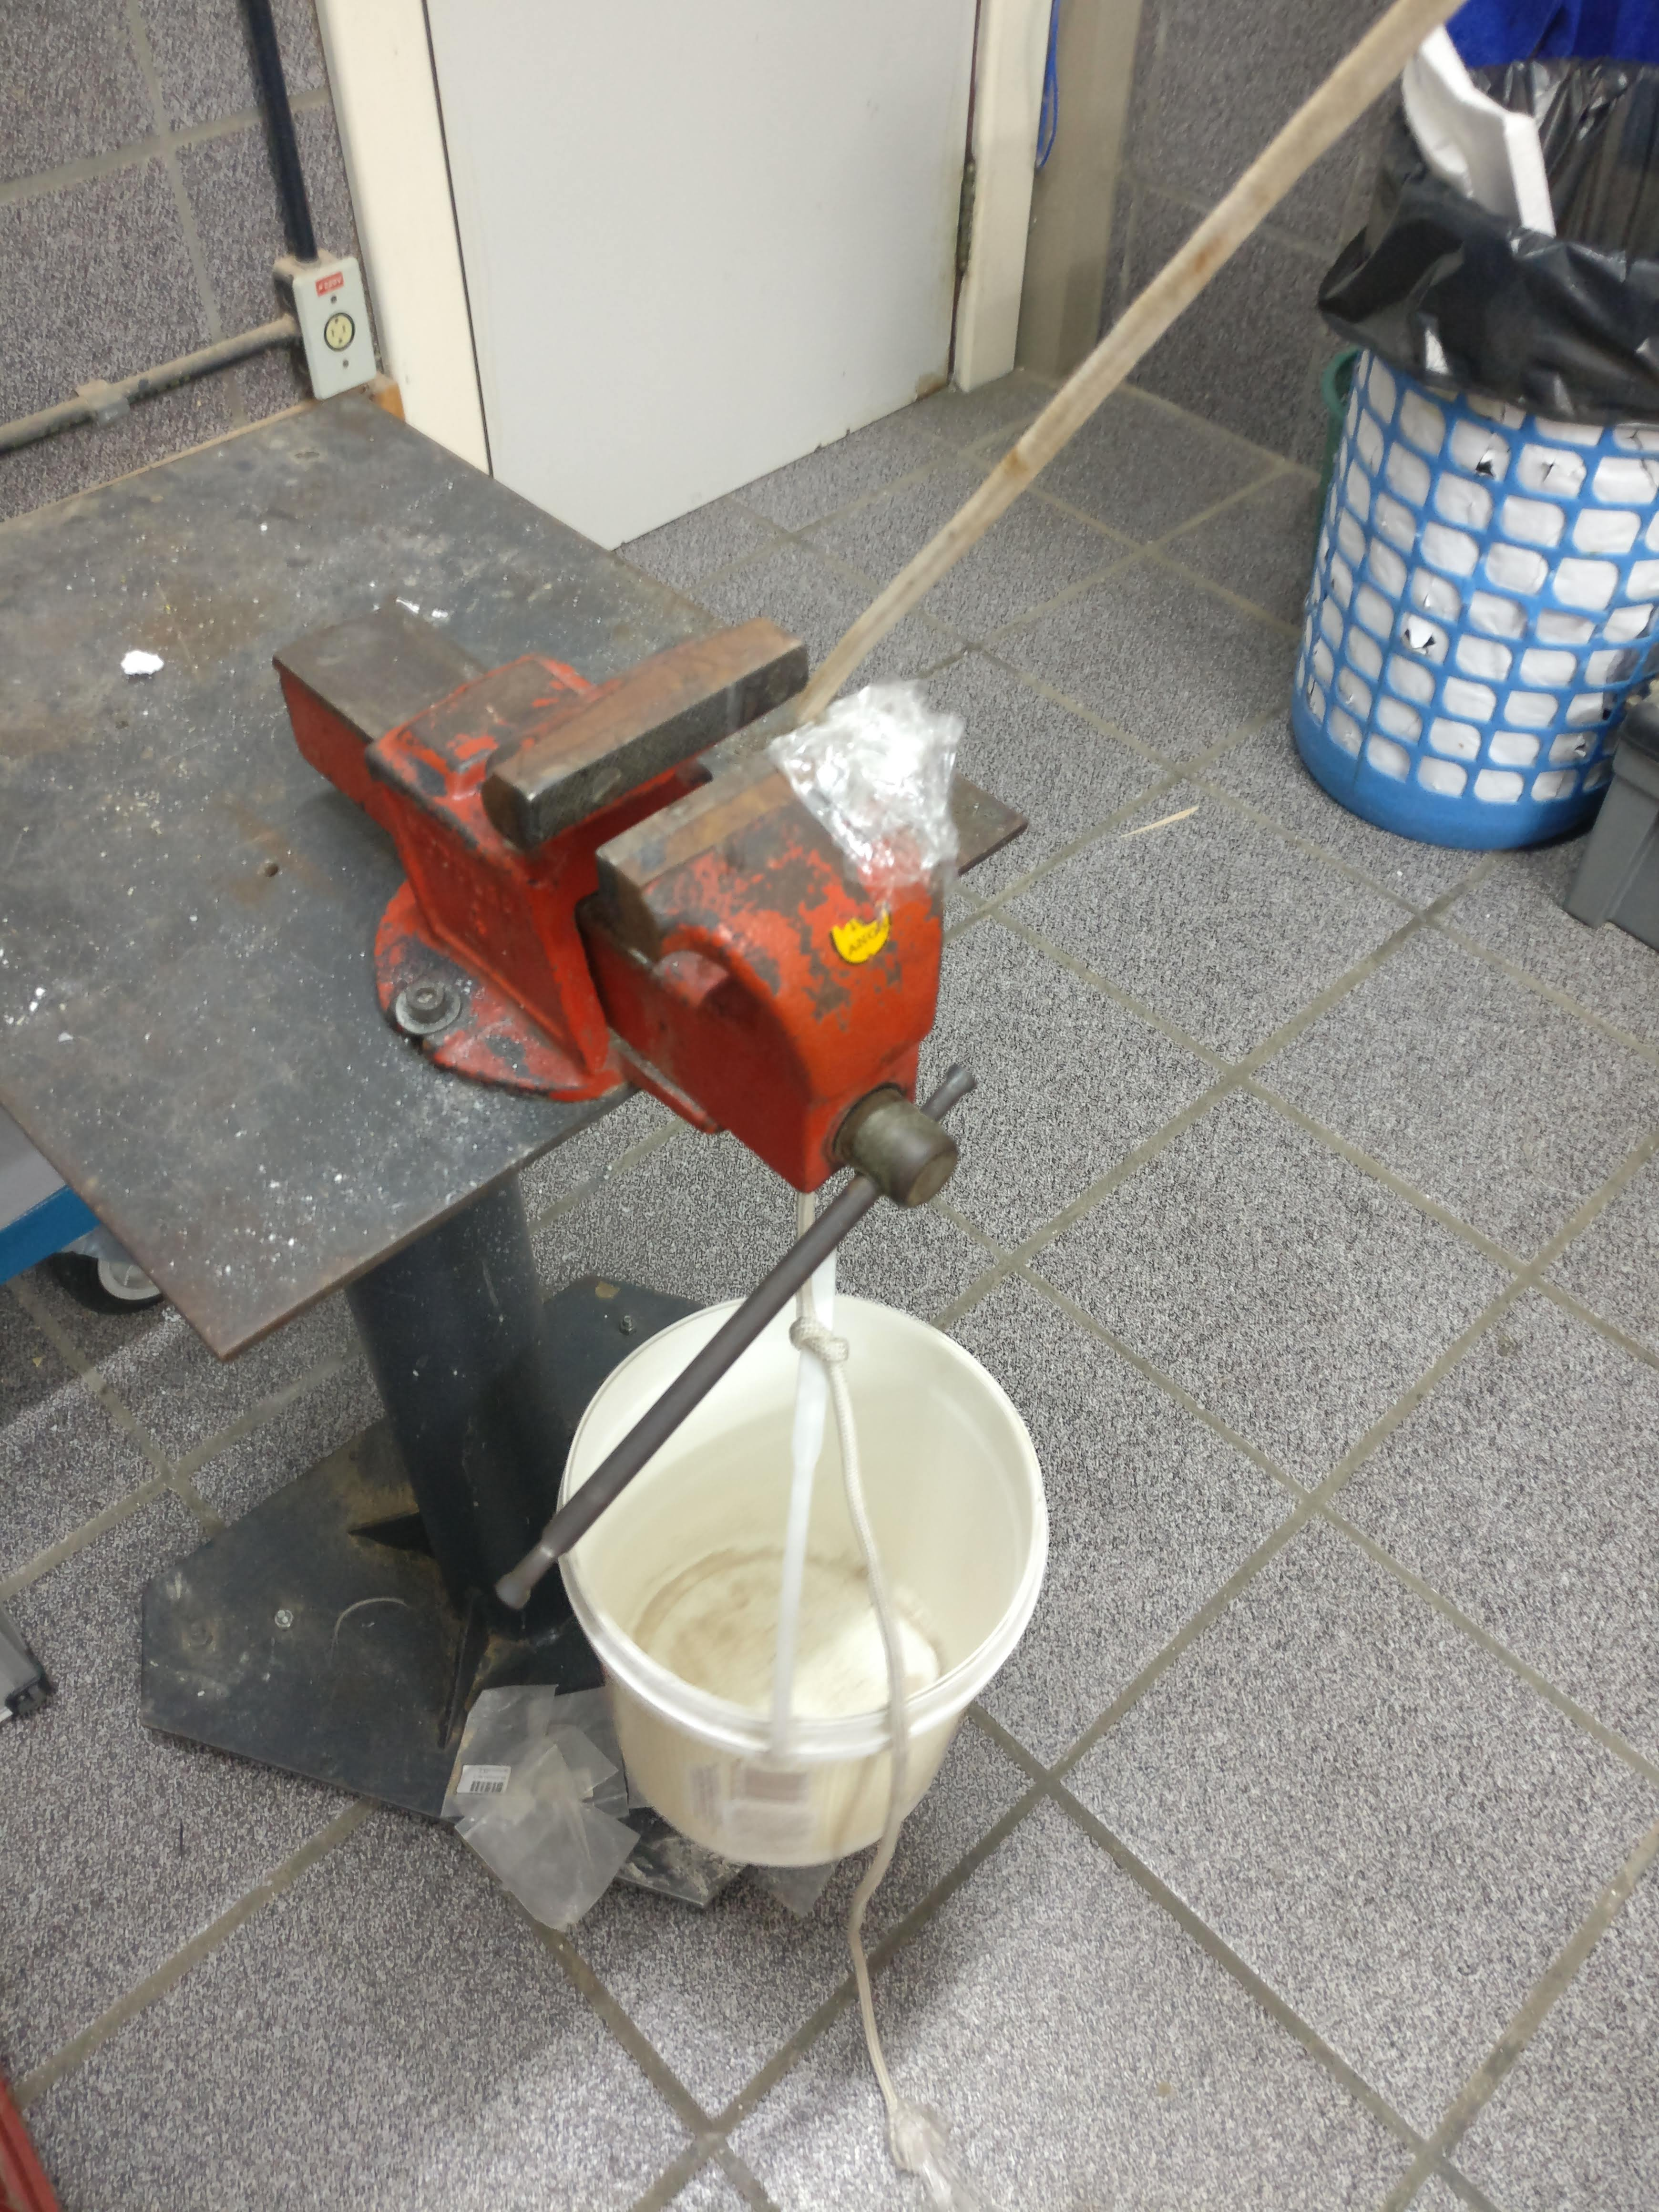
\includegraphics[width=0.4\columnwidth]{figuras/calibracao/polia2.jpg}}
        \label{polias_2}
\end{figure}

Cada peso foi avaliado com uma balança de precisão com resolução de 1g e erro de +-0.5g, mostrada na figura \ref{fig:balanca_precisao}.

\begin{figure}[!ht]
    \centering
    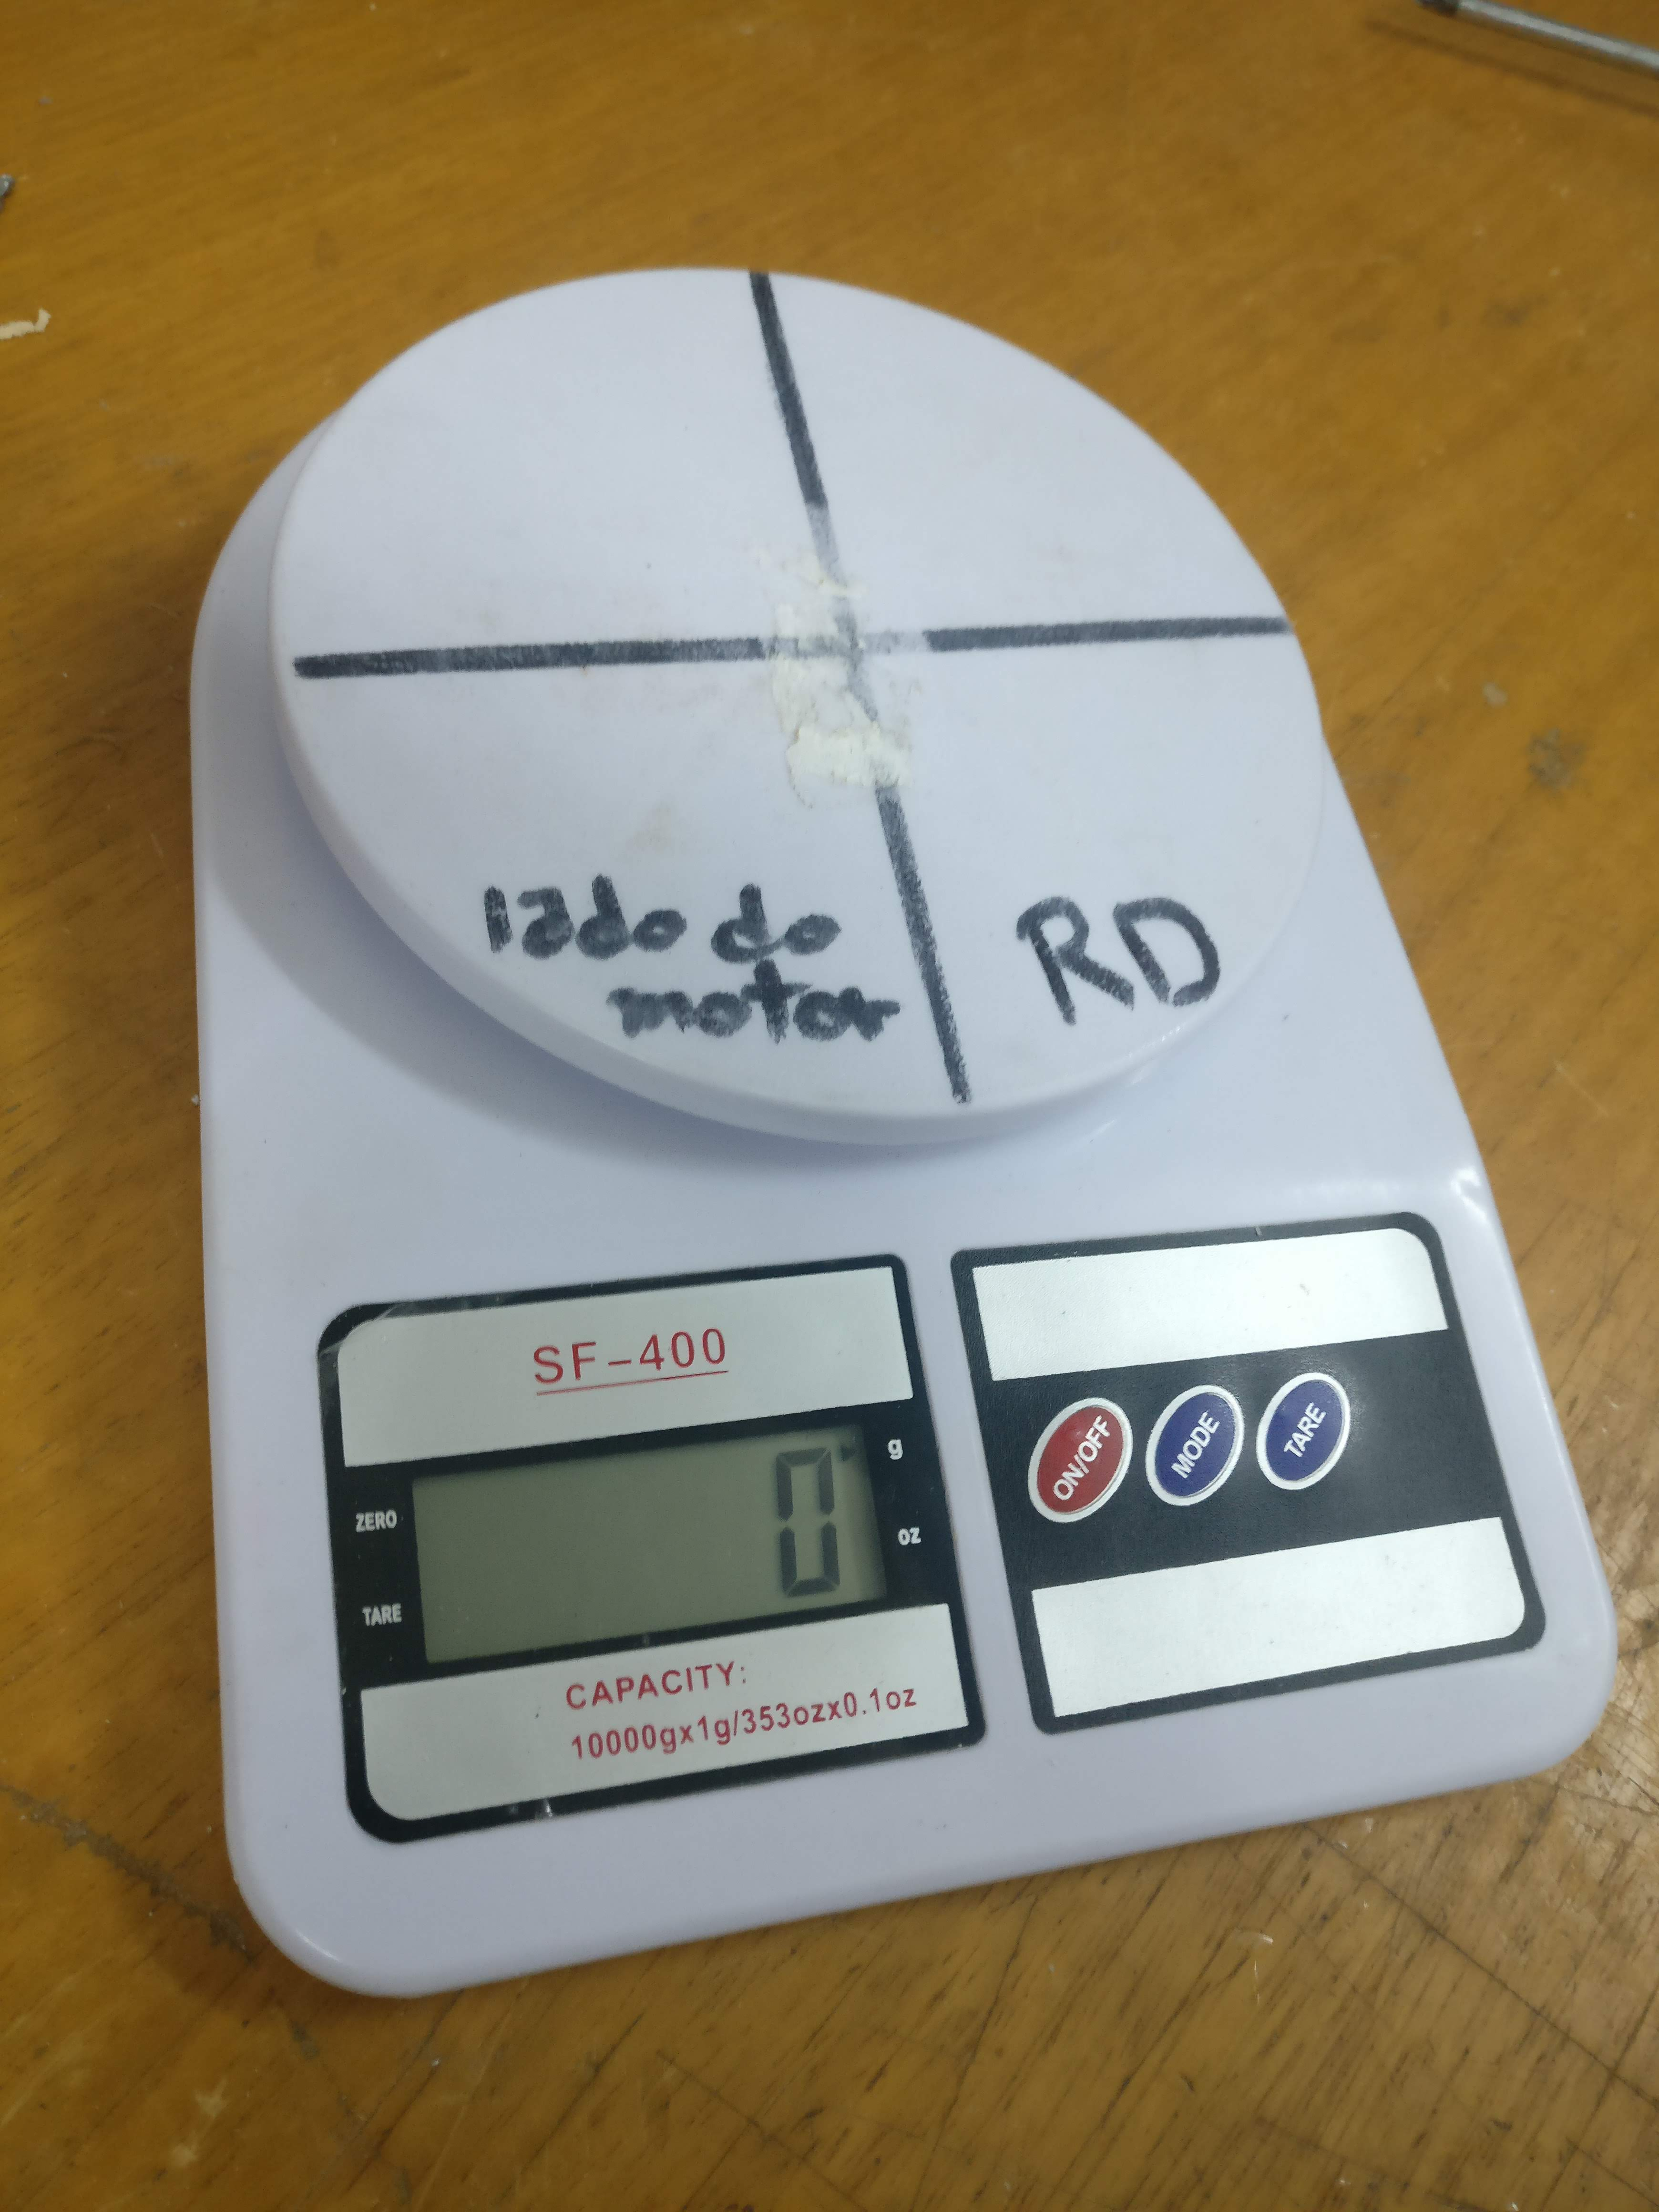
\includegraphics[width=.4\linewidth]{figuras/calibracao/balanca_precisao.jpg}
    \caption{Balança de precisão utilizada para aferição dos pesos de calibração. Fonte: O autor.}
    \label{fig:balanca_precisao}
\end{figure}

Cada célula foi inicialmente carregada apenas com o balde onde os pesos eram colocados. As células eram então zeradas e o valor respectivo a 0g era então anotado.
Para cada nova carga imposta, um vetor de 100 pontos eram coletado, com a média, desvio padrão e coeficiente de variação dos mesmos extraída.

Notou-se já na calibração da primeira célula que o coeficiente de variação (CV) estava alto, chegando a mais de 4\%, e quando deixada a variar a medida demorava minutos até estabilizar. Foram então impostos carregamentos e descarregamentos sucessivos, e uma histerese com CV que chegava aos 18\% entre os diferentes ciclos estava presente. Esta histerese porém não se apresentava quando o sistema de polias não era utilizado. A solução encontrada foi realizar a calibração sem o sistema de polias, invertendo as células e carregando-as diretamente. Desta forma o CV máximo das 100 aquisições ficou abaixo de 0.2\% para todas as células, com as mesmas estabilizando em décimos de segundo. Os dados adquiridos se encontram na tabela \ref{tab:calib_celulas}.

\begin{table}[]
\centering
\resizebox{\textwidth}{!}{\begin{tabular}{llllllllllll}
Massa {[}g{]} & Peso {[}N{]} &  & \begin{tabular}[c]{@{}l@{}}Célula \\ Horizontal\end{tabular} & \begin{tabular}[c]{@{}l@{}}Célula\\ Frontal\\ Esquerda\end{tabular} & \begin{tabular}[c]{@{}l@{}}Célula\\ Frontal\\ Direita\end{tabular} & \begin{tabular}[c]{@{}l@{}}Célula\\ Traseira\\ Esquerda\end{tabular} & \begin{tabular}[c]{@{}l@{}}Célula\\ Traseira\\ Direita\end{tabular} &  & \begin{tabular}[c]{@{}l@{}}Arrasto\\ (max)\end{tabular} & \begin{tabular}[c]{@{}l@{}}Arrasto\\ (min)\end{tabular} & \begin{tabular}[c]{@{}l@{}}Arrasto\\ (medio)\end{tabular} \\
 &  &  &  &  &  &  &  &  &  &  &  \\
0 & 0.0 &  & -420 & -59 & 0 & 40 & -15 &  & 15128 & -14256 & 436 \\
142 & 1.4 &  & 62860 & 31544 & 31548 & 31580 & 31222 &  & 68497 & 45658 & 57078 \\
208 & 2.0 &  & 92192 & 46222 & 46266 & 46170 & 45652 &  & 101682 & 73246 & 87464 \\
352 & 3.5 &  & 155114 & 77814 & 77839 & 77632 & 76934 &  & 166984 & 147624 & 157304 \\
491 & 4.8 &  & 217264 & 109054 & 109067 & 108810 & 107894 &  & 237679 & 190734 & 214207 \\
1194 & 11.7 &  & 525814 & 264322 & 264342 & 263620 & 261004 &  & 499000 & 450000 & 474500 \\
1995 & 19.6 &  & 878342 & 441205 & 440885 & 439952 & 435844 &  & 831000 & 778000 & 804500 \\
3541 & 34.7 &  & 1562200 & 784432 & 784167 & 781870 & 775270 &  & 1580000 & 1382000 & 1481000 \\
6344 & 62.2 &  & 2794214 & 1404280 & 1403660 & 1400334 & 1387765 &  & 2770000 & 2532000 & 2651000 \\
9362 & 91.8 &  & 4099312 & 2063650 & 2061925 & 2058910 & 2043574 &  & 4032970 & 3916820 & 3974895
\end{tabular}}
\caption{Medições das massas de calibração e respectivas leituras das células.}
\label{tab:calib_celulas}
\end{table}

\begin{figure}[!ht]
    \centering
    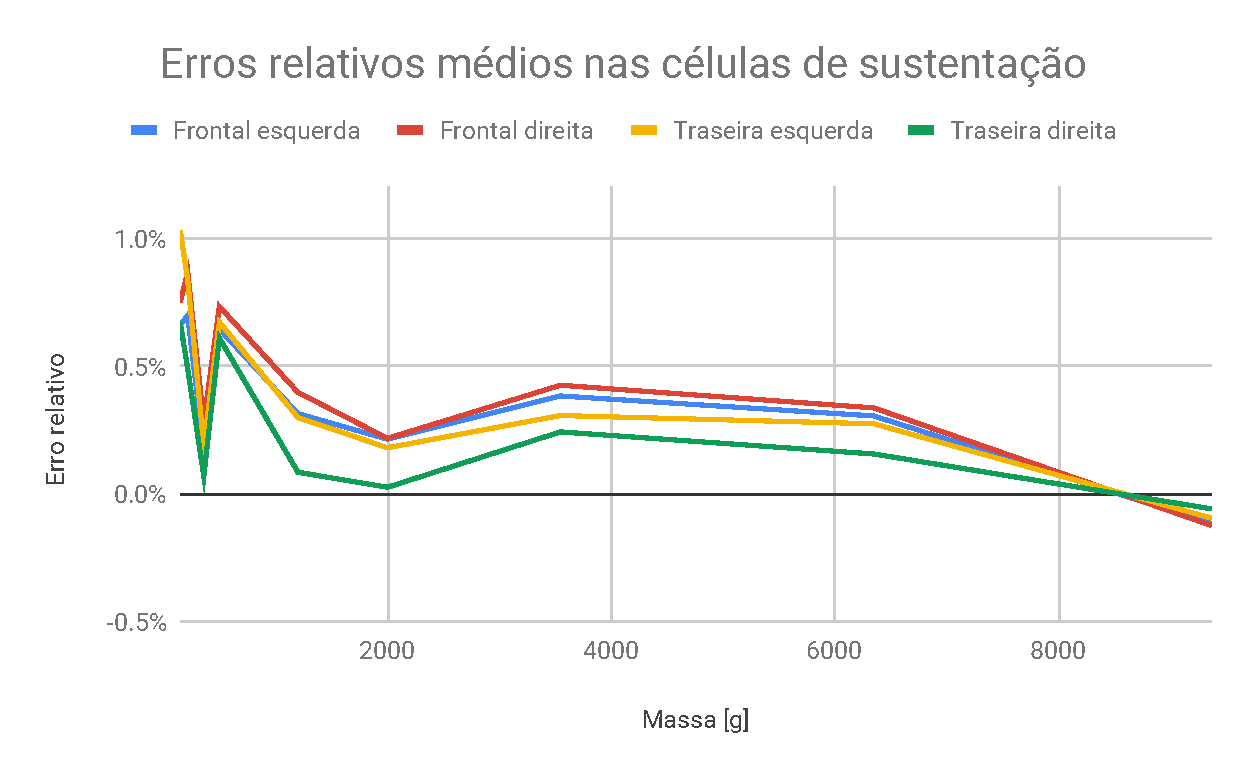
\includegraphics[width=.8\linewidth]{figuras/calibracao/plot_erro_sustentacao.pdf}
    \caption{Erro relativo médio para medições das células de sustentação. Fonte: O autor.}
    \label{fig:curva_erros_sustentacao}
\end{figure}

Outro problema foi então encontrado nesta calibração. Mesmo sem o uso do sistema de polias, uma histerese que chegava a 40\% para baixas cargas e se mantinha perto dos 10\% para as cargas mais altas estava presente na medição de arrasto. Foi realizada uma tentativa de calibração da célula de arrasto instalando-a na vertical, não mais em série com as guias lineares, e a calibração da mesma não apresentou mais histerese, tendo resultados compatíveis com os das demais células.

A hipótese mais provável é de que a histerese seja resultado do atrito nas guias lineares, tornando portanto esta solução pior que a alternativa sem as guias. A mudança de uma solução para a outra porém exigiria compra de novas células, além da modificação da placa de aquisição de sinais, bem como de seu código, ambos adaptados para o uso de apenas uma célula de arrasto. Por este motivo não foi realizada a mudança na solução, mas a mesma é recomendada com máxima prioridade para uma modificação futura do projeto.

Para que o uso da bancada tenha maior fidelidade à realidade, a célula de arrasto foi recolocada em sua posição original e a calibração da mesma foi realizada nesta configuração (em série com as guias lineares), com a histerese presente. Como pode-se ver na figura \ref{fig:curva_erros_arrasto}, deve-se esperar desvios de até 22\% para cargas de até 1,2kg e de aproximadamente 6\% para cargas maiores.

\begin{figure}[!ht]
    \centering
    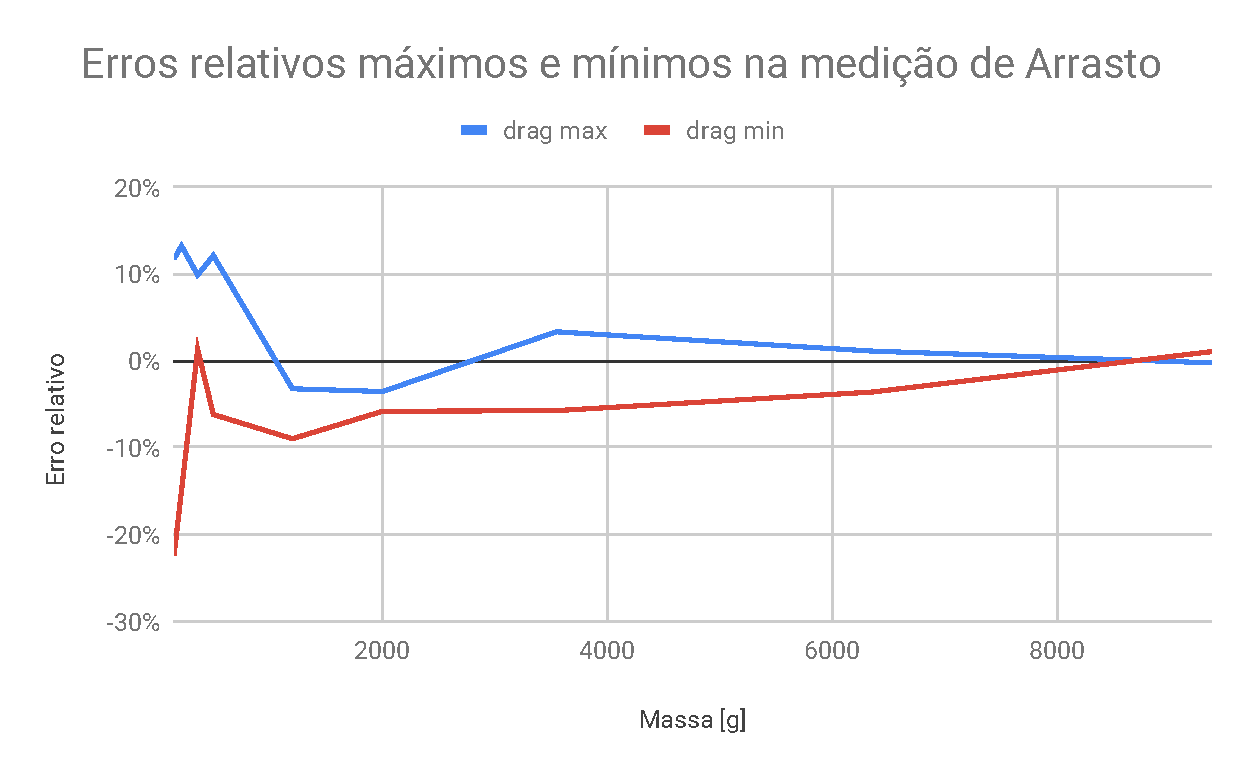
\includegraphics[width=.8\linewidth]{plots/celulas_plot_1.pdf}
    \caption{Erro relativo máximo e mínimo para medições de arrasto. Fonte: O autor.}
    \label{fig:curva_erros_arrasto}
\end{figure}

Foram então plotados os valores médios de leitura contra cada carregamento e uma regressão linear foi feita para cada célula. A função de transferência para uma das células de sustentação se encontra na figura \ref{fig:curva_celula_vertical}. Os coeficientes para todas as células se encontram na tabela \ref{tab:coeficientes_celulas}.

\begin{figure}[!ht]
    \centering
    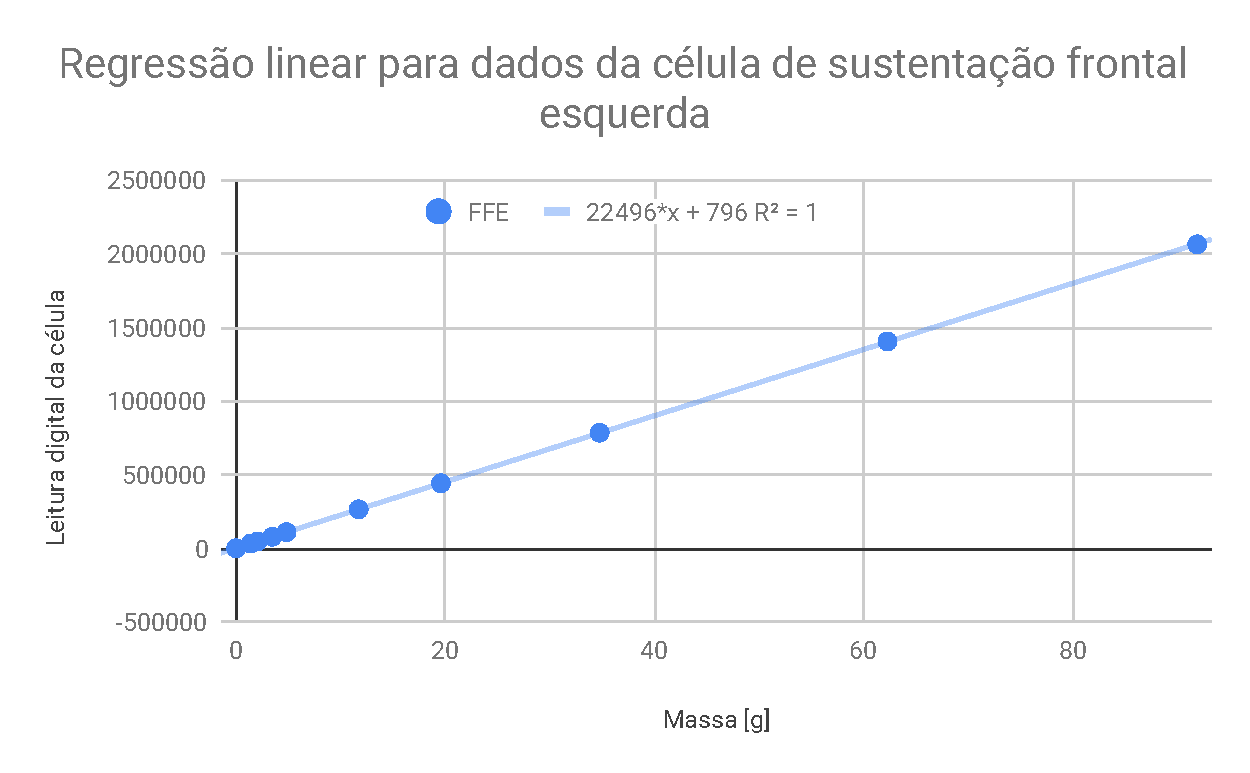
\includegraphics[width=.8\linewidth]{figuras/calibracao/plot_regressao_sustentacao.pdf}
    \caption{Pontos adquiridos e curva calibrada para uma das células de medição de forças verticais. Fonte: O autor.}
    \label{fig:curva_celula_vertical}
\end{figure}


\begin{table}[]
\centering
\resizebox{\textwidth}{!}{\begin{tabular}{lllllllllll}
 &  & \begin{tabular}[c]{@{}l@{}}Célula\\ Horizontal\end{tabular} & \begin{tabular}[c]{@{}l@{}}Célula\\ Frontal\\ Esquerda\end{tabular} & \begin{tabular}[c]{@{}l@{}}Célula\\ Frontal\\ Direita\end{tabular} & \begin{tabular}[c]{@{}l@{}}Célula\\ Traseira\\ Esquerda\end{tabular} & \begin{tabular}[c]{@{}l@{}}Célula\\ Traseira\\ Direita\end{tabular} &  & \begin{tabular}[c]{@{}l@{}}Arrasto\\ (max)\end{tabular} & \begin{tabular}[c]{@{}l@{}}Arrasto\\ (min)\end{tabular} & \begin{tabular}[c]{@{}l@{}}Arrasto\\ (medio)\end{tabular} \\
Coef. Angular &  & 44708 & 22496 & 22479 & 22439 & 22264 &  & 44006 & 42192 & 43099 \\
Coef. Linear &  & 2365 & 796 & 914 & 748 & 432 &  & 10243 & -27835 & -8796
\end{tabular}}
\caption{Coeficientes de calibração das células}
\label{tab:coeficientes_celulas}
\end{table}

Foi também plotado o erro das curvas estimadas por regressão contra os valores do teste, obtendo o erro relativo a cada carregamento. A regressão utilizando apenas o coeficiente angular apresentou diferença menor que 0.01\% em relação a regressão com o coeficiente linear também presente, de modo que a primeira forma de regressão foi utilizada. A vantagem desta opção é diminuir o volume de dados de calibração passados para o código da bancada.

Como pode ser visto, na faixa de medição para baixos pesos o desvio relativo da medida é maior, mas ainda bastante baixo, com teto para as células de sustentação de 1.06\% para valores inferiores a 1,2kg e 0.59\% para valores superiores. O erro médio de todas as medições foi de 0.4\%.

% \subsection{Calibração integrada das células}

% Em seguida foi realizada a calibração conjunta de cargas. Foram impostas diversas combinações de carga de arrasto e sustentação de forma simultânea visando avaliar o erro devido ao acoplamento das cargas, isto é, o quanto uma carga influencia na leitura da outra. Ums proposta de correçao para este acoplamento seria realizada segundo a equação X.

% \begin{equation}
%     L = A1*L_{Raw} - A2*D_{Raw}
% \end{equation}

% \begin{equation}
%     D = A3*D_{Raw} - A4*L_{Raw}
% \end{equation}

% Os resultados para as curvas com e sem cargas simultaneas se encontram plotados nas figuras X e X.

% \begin{figure}[!ht]
%     \centering
%     
\includegraphics[width=.8\linewidth]{figuras/outras/placeholder.png}
%     \caption{Curva de sustentaçao com e sem carga de arrasto. Fonte: O autor.}
%     \label{fig:placeholder}
% \end{figure}

% Pode-se verificar para o caso da mediçao de sustentaçao que existe um desvio que fica entre 0.3\% e 1.74\% entre as curvas medidas com e sem cargas simultâneas, indicando que de fato existe um acoplamento entre as medições. Para o caso da leitura de arrasto, porém, o desvio devido a histerese é uma ordem de grandeza maior que os efeitos esperados para o acoplamento, mascarando os resultados do mesmo. Deste modo, a correçao por acoplamento ficou bastante comprometida, com resultados que nao trariam ganho em precisao, e portanto foi descartada.

\subsection{Calibração do tubo de Pitot e sonda de AoA}

\begin{figure}[!ht]
    \centering
    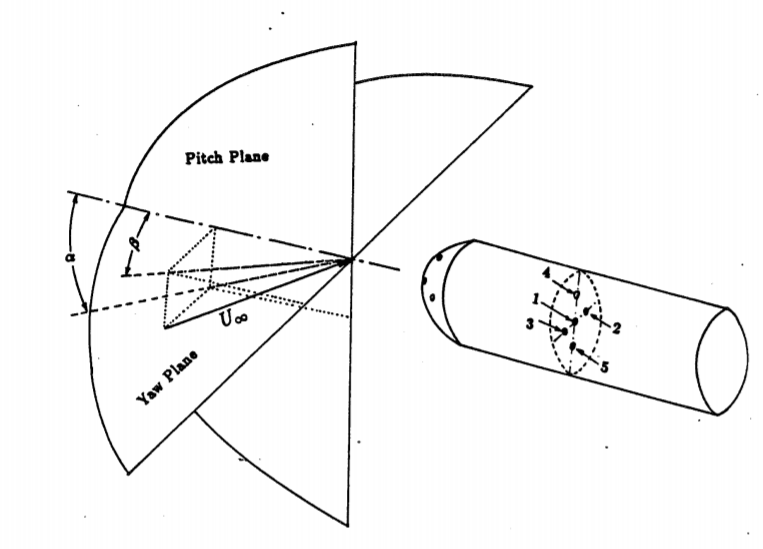
\includegraphics[width=.8\linewidth]{figuras/outras/5holepitot.png}
    \caption{Sonda de ângulo de ataque de 5 tomadas. A tomada numero 6, de pressão estática, é posicionada lateralmente ao tubo. Fonte: \cite{lee1986calibration}}
    \label{fig:5_hole_probe}
\end{figure}

Dada a maior flexibilidade e pouco aumento de custo, foram utilizados apenas Pitots de múltiplas tomadas na bancada, ignorando-se as tomadas diferenciais quando da não necessidade de medição de ângulo de ataque. 

As calibrações dos tubos de Pitot de múltiplas tomadas foram realizadas no túnel de vento da UFSC variando-se discretamente o ângulo de ataque de -20 a 20 graus, com passo de 2 graus, utilizando o disco de medição angular presente na balança do túnel de vento. O teste foi realizado para 7 velocidades de escoamento no túnel, apresentadas ao final deste capitulo. 

\begin{figure}[!ht]
    \centering
    \caption{Sistema utilizado para calibração da sonda de ângulo de ataque. Fonte: O autor.}
        \subfloat[Sonda instalada em adaptador para o túnel de vento, com caixa da IMU acoplada.]{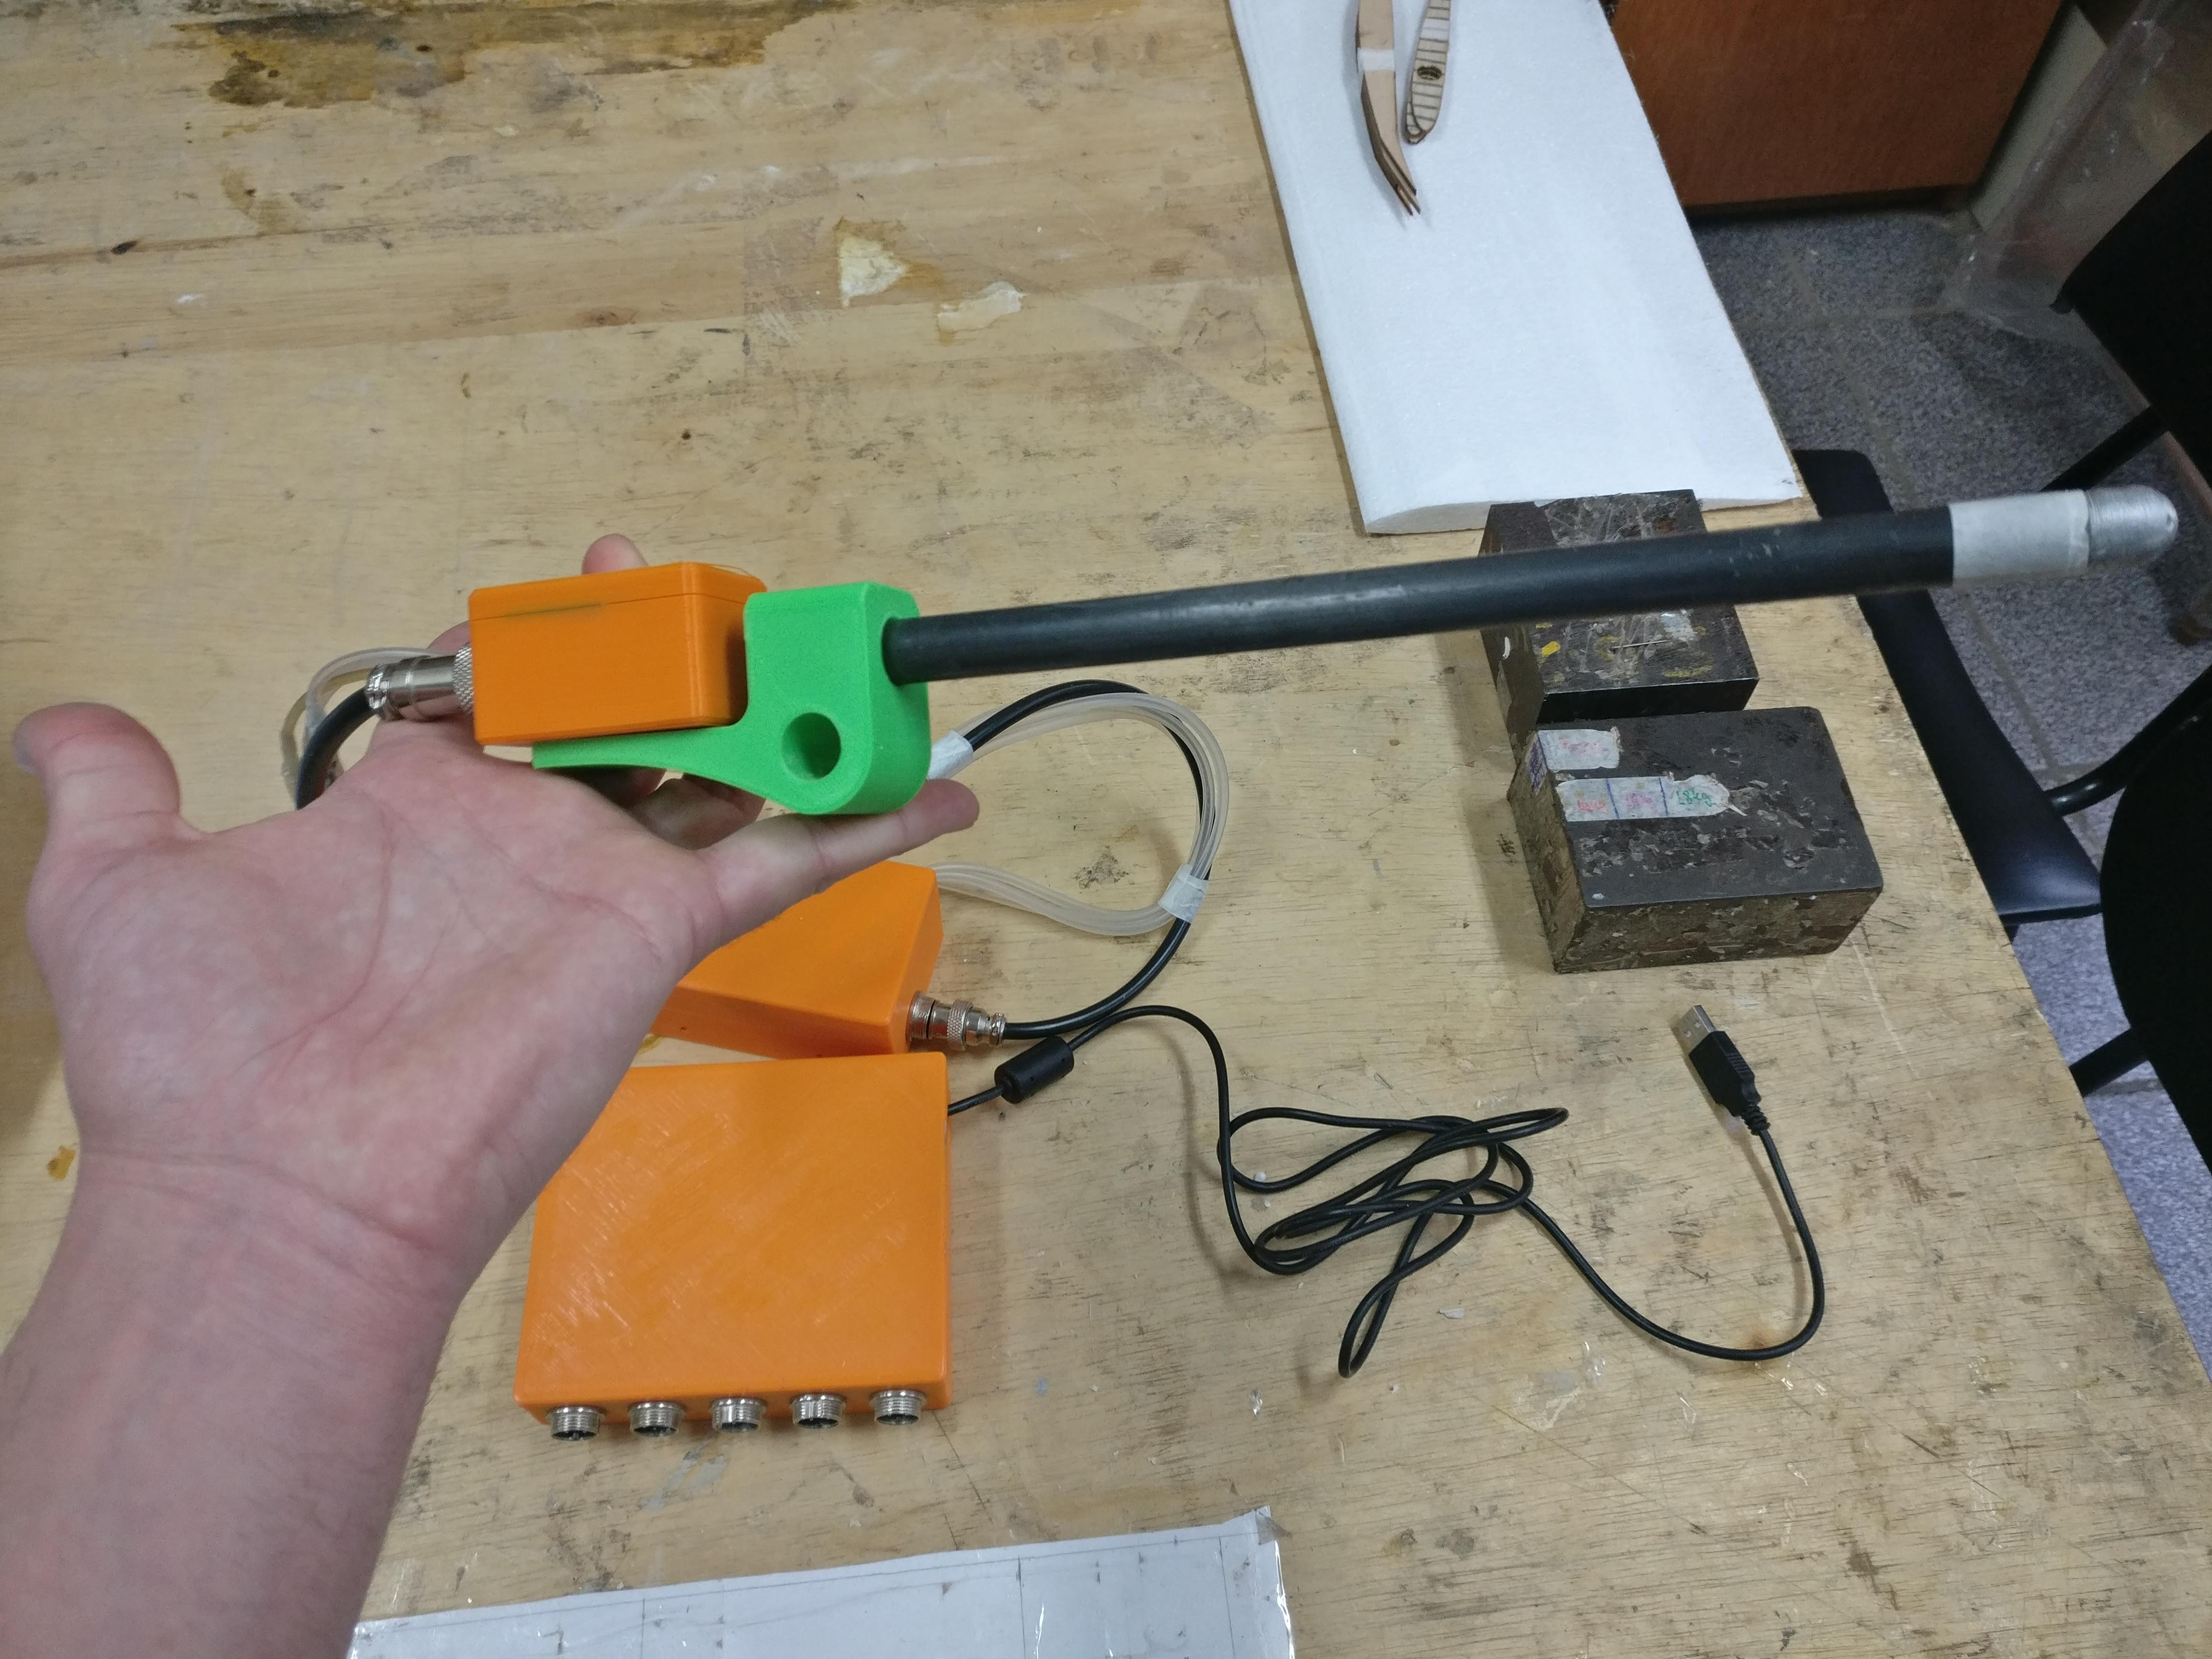
\includegraphics[width=0.4\columnwidth]{figuras/calibracao/dispositivo_sonda.jpg}}
        \label{sonda_tunel_1}
        \qquad
        \subfloat[Sistema instalado no túnel de vento.]{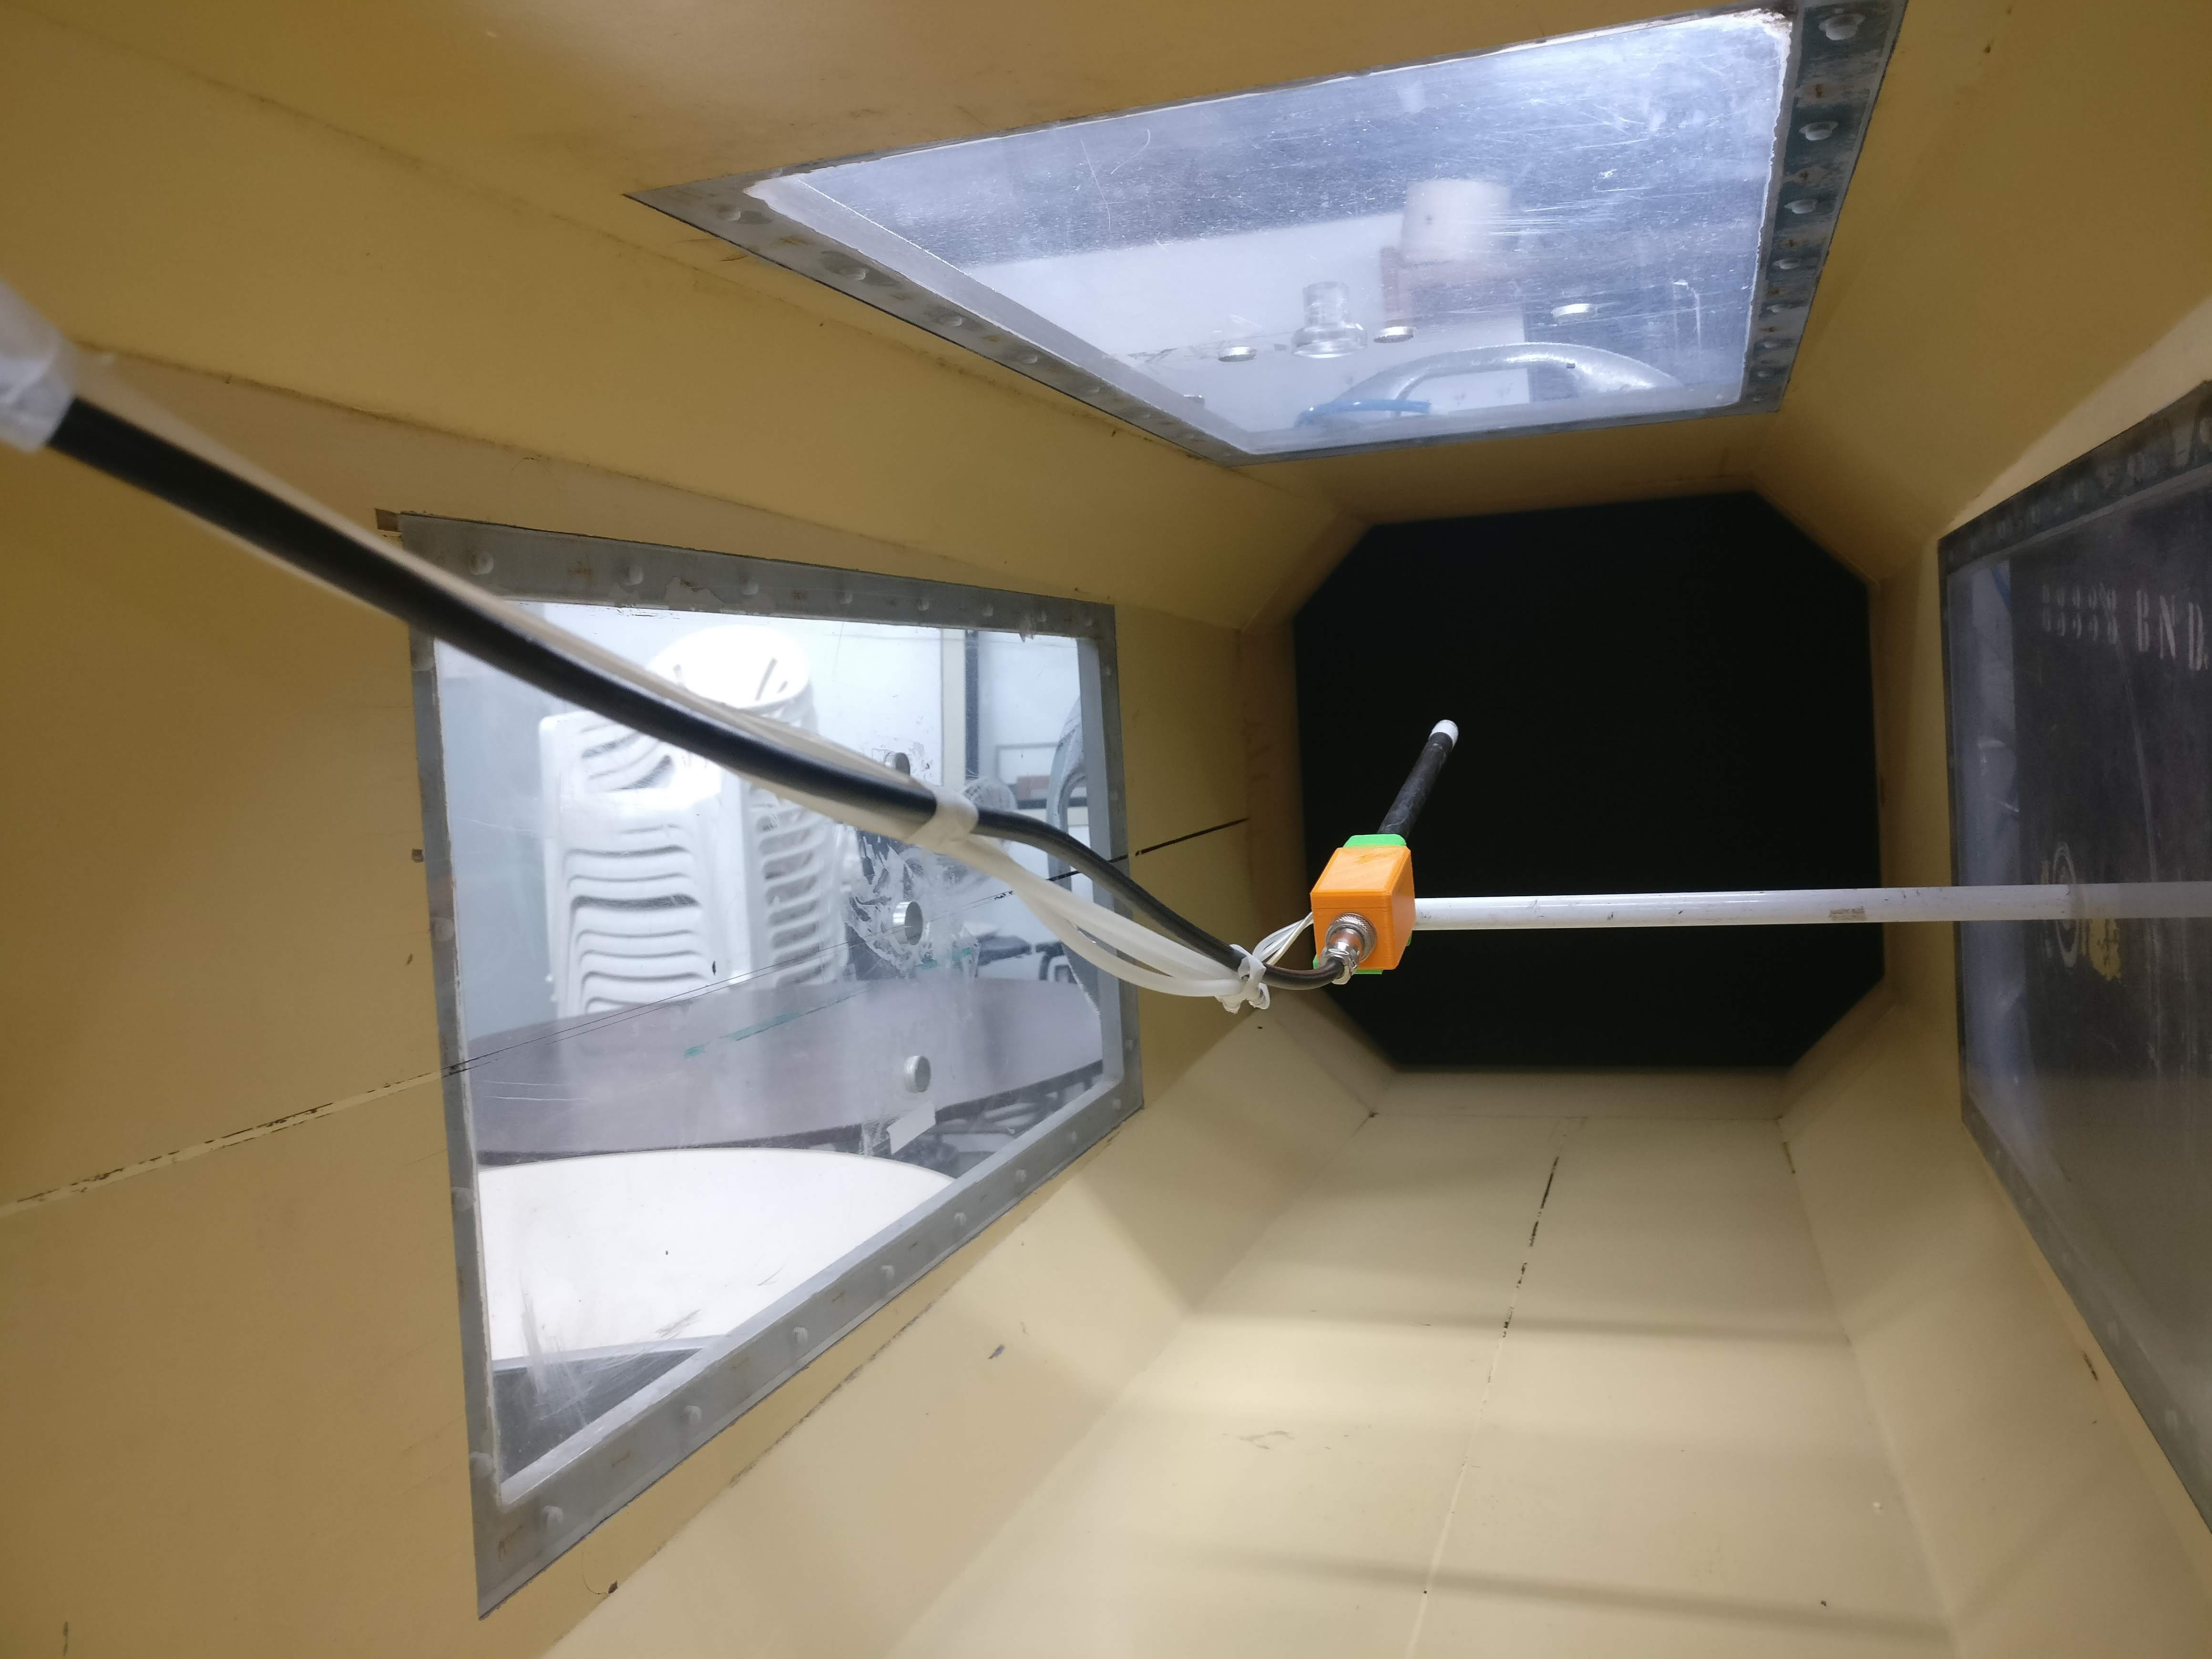
\includegraphics[width=0.4\columnwidth]{figuras/calibracao/sonda_tunel.jpg}}
        \label{sonda_tunel_2}
\end{figure}

Para aumentar a agilidade no teste e no pós-processamento dos dados foi instalada uma IMU na sonda, medindo-se assim o ângulo de ataque da mesma através da equação \ref{eq:acc_angle}. Foram realizadas medições de pressão diferencial nos pares de tomadas 1-6 e 4-5, denominadas respectivamente pressão-dinâmica e pressão-diferencial.

\begin{equation}
    \alpha = \arctan \frac{Acc_y}{\sqrt{Acc_x^2+Acc_y^2}}   
    \label{eq:acc_angle}
\end{equation}


Segundo \cite{borges2008desenvolvimento} o ângulo do escoamento é proporcional à razão $\frac{\Delta P}{q}$ onde $\Delta P$ é a diferença de pressão entre as tomadas alinhadas com o plano de medição (picada ou guinada) e $q$ é a pressão dinâmica do escoamento.

% Para a normalização dos dados \cite{lee1986calibration} recomenda o referenciamento em relação a media das pressões nas quatro tomadas laterais (2, 3, 4, 5), conforme as equações X, Y e Z.

% \begin{equation}
%     C_{P_{pitch}} = \frac{P_4 - P_5}{P_1 - P_{ref}}
% \end{equation}
% \begin{equation}
%     C_{P_{total}} = \frac{P_1 - P_{total}}{P_1 - P_{ref}}
% \end{equation}
% \begin{equation}
%     C_{P_{static}} = \frac{P_{ref} - P_{static}}{P_1 - P_{ref}}
% \end{equation}
% \begin{equation}
%     P_{ref} = \frac{P_2 + P_3 + P_4 + P_5}{4}
% \end{equation}

Para o presente caso as tomadas de yaw (2 e 3) nao foram utilizadas, dado que o interesse é apenas na mediçao do ângulo de ataque.

% A pressão estática é medida por um transdutor de pressão atmosférica, presente na IMU, enquanto a pressão total do escoamento é a soma da pressão-dinamica (diferença das tomadas 1 e 6) quando $\alpha$ é igual a 0 graus com a pressão estática.

Os resultados da medição de $\frac{\Delta P}{q}$ por $\alpha$ se encontram na figura \ref{fig:Deltapq_alpha_plot}.

\begin{figure}[!ht]
    \centering
    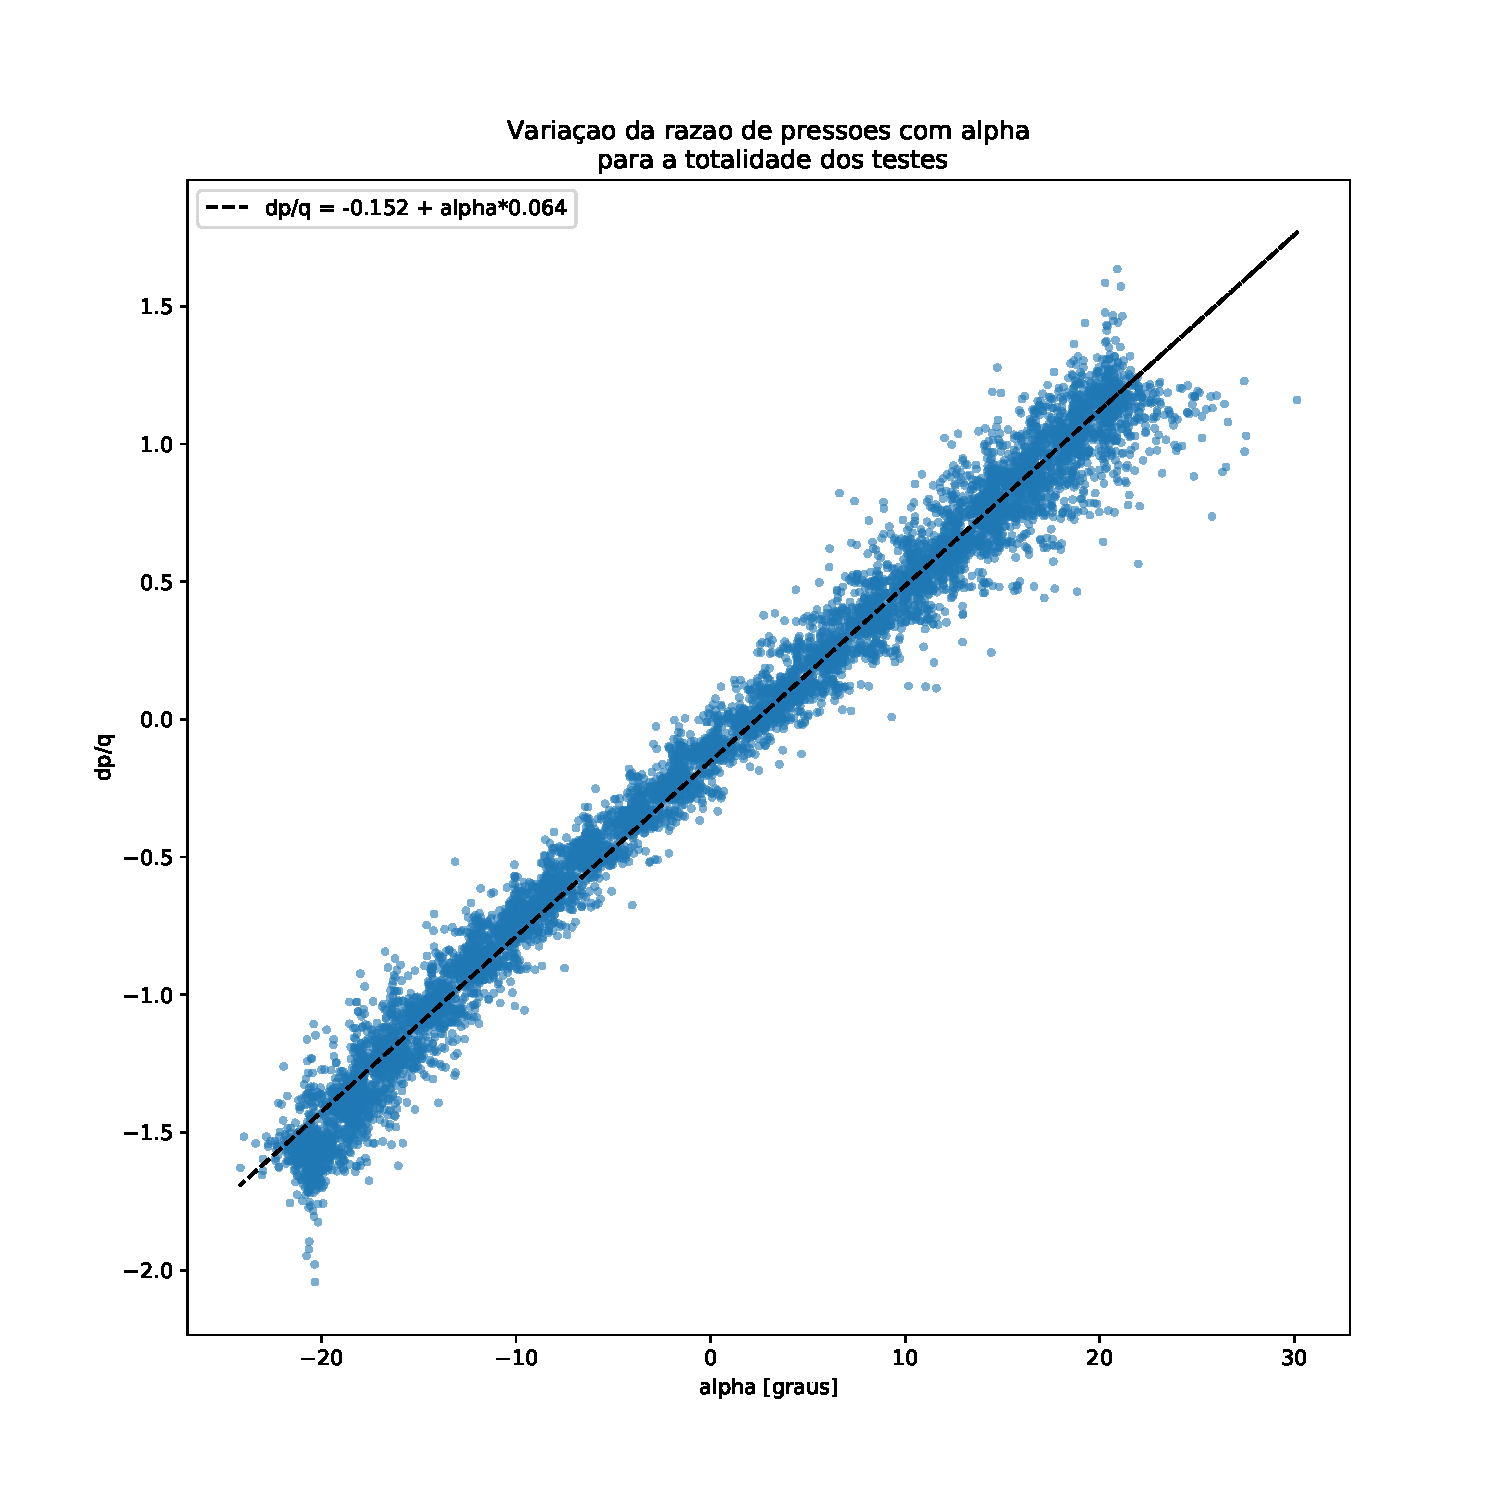
\includegraphics[width=.7\linewidth]{figuras/calibracao/dp-q_plot.pdf}
    \caption{Medições de $\frac{\Delta P}{q}$ por $\alpha$ no teste em túnel de vento. Neste gráfico se encontram presentes os pontos adquiridos para todas as velocidades de escoamento testadas no túnel de evento. Fonte: O autor.}
    \label{fig:Deltapq_alpha_plot}
\end{figure}

Foi realizada uma regressão linear neste gráfico \citep{borges2008desenvolvimento}. O erro máximo da linearização e o erro médio quadrático para ângulos entre -15 e +15 graus são respectivamente 1.32 graus e 0.42 graus.

\begin{equation}
    \alpha = 2.34 + 15.45 * \frac{\Delta P}{q}
\end{equation}

O modulo do vetor velocidade pode então ser calculado pela equação \ref{eq:velocity_q}. 

\begin{equation}
    U = \sqrt{\frac{2q}{\rho}}
    \label{eq:velocity_q}
\end{equation}

% TABELA COM CONDICOES ATMOSFERICAS
% PRESSAO 101.8kPa
% Temp 16C
% Umidade 70\%
% Densidade estimada 1.227

Para averiguação do valor verdadeiro da velocidade do escoamento, tomado como referencia para caibração, foi utilizado um anemômetro de fio quente. O gráfico \ref{fig:U_alpha} mostra o valor verdadeiro da velocidade e a velocidade medida pela sonda, com variação do ângulos de ataque de -20 a 20 graus.

\begin{figure}[!ht]
    \centering
    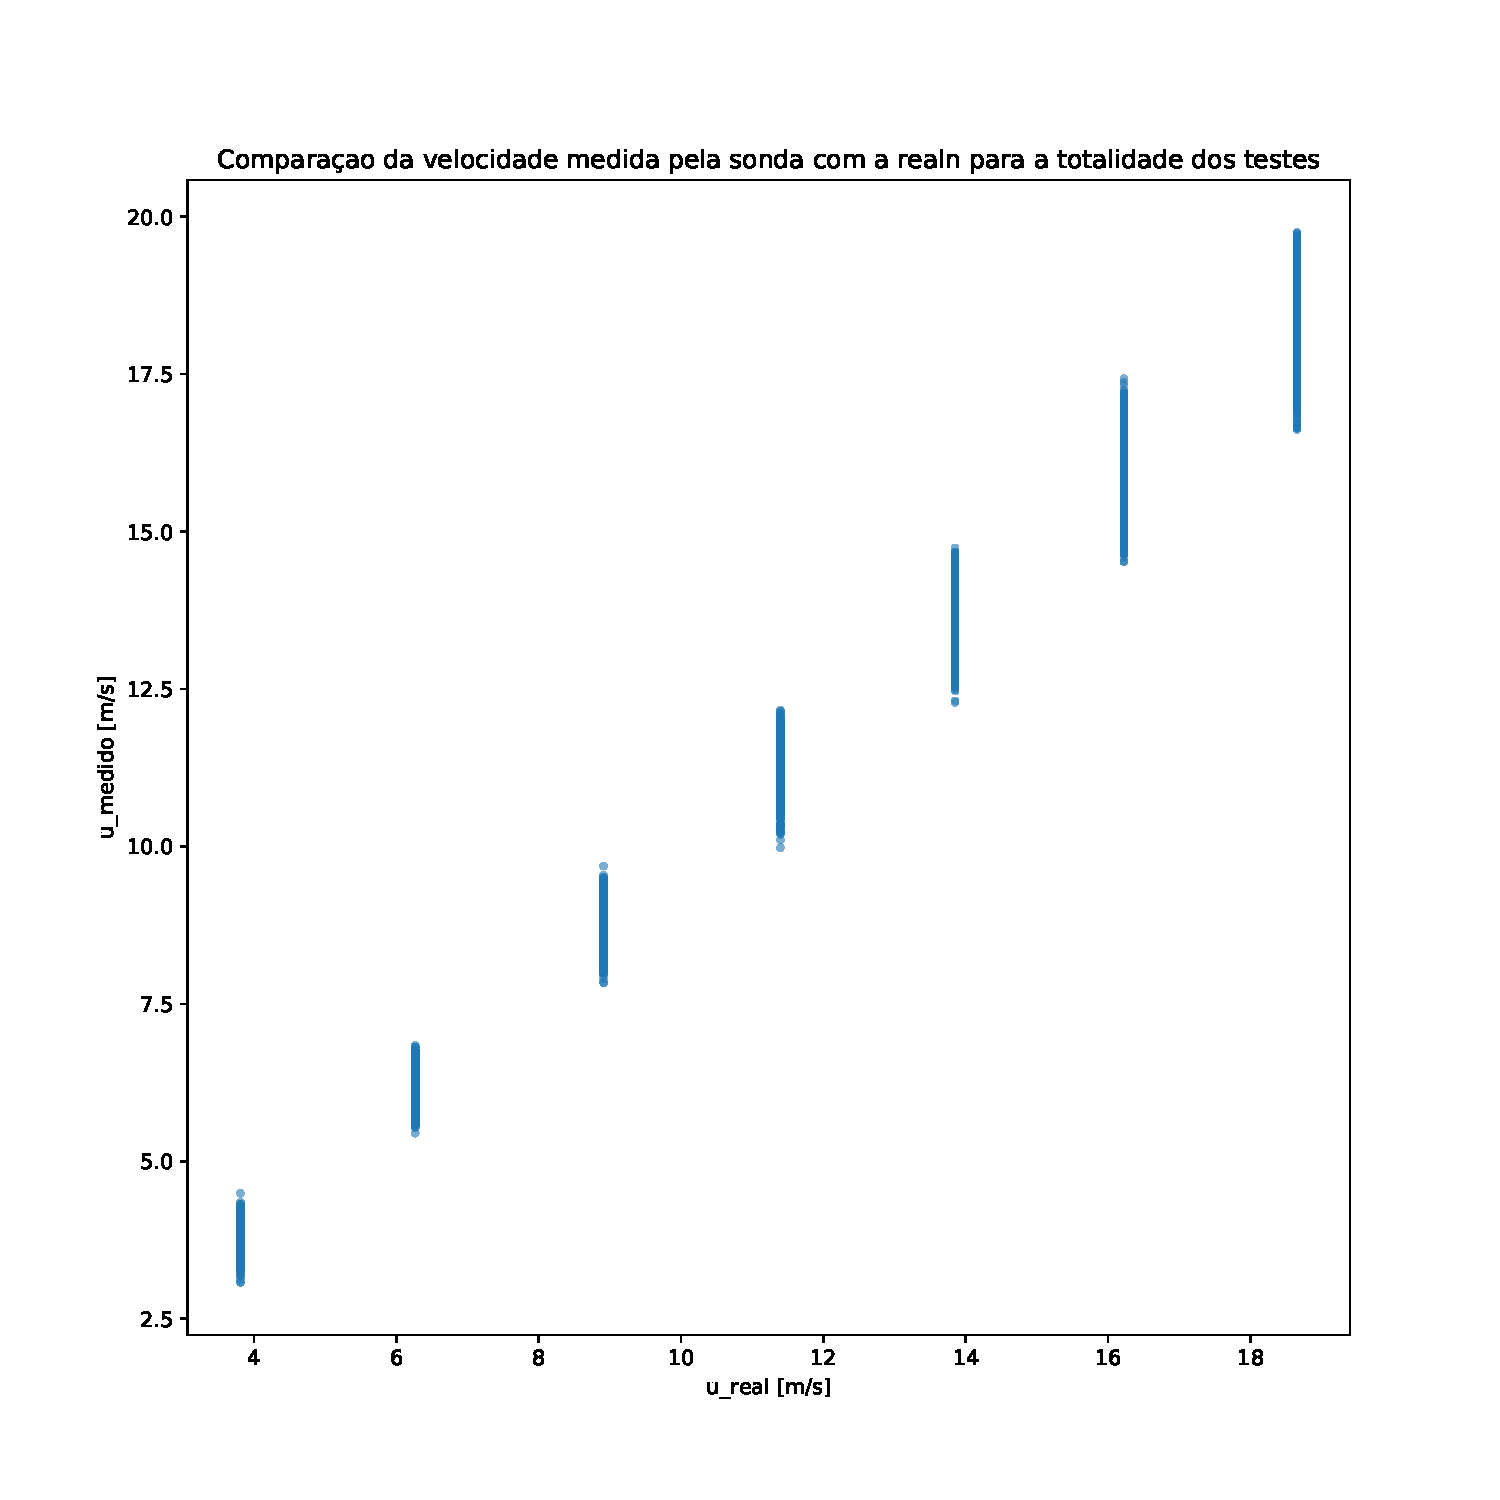
\includegraphics[width=.8\linewidth]{figuras/calibracao/u_ver_plot.pdf}
    \caption{Velocidade medida através da sonda $vs$ velocidade medida por anemômetro de fio quente. Fonte: O autor.}
    \label{fig:U_alpha}
\end{figure}

O erro máximo da velocidade medida e o erro médio quadrático para cada velocidade de escoamento do túnel de vento, para ângulos entre -15 e +15 graus foram de respectivamente 12.4\% e 1.8\%.

\section{Testes}

Uma serie de testes foi realizada inicialmente de forma mais rápida visando-se buscar melhorias a serem feitas na bancada, seja na parte mecânica, eletrônica ou de software. Estes testes se deram simultaneamente ao projeto e auxiliariam em diversas melhorias do projeto e do processo de execução dos testes, entre eles:

\begin{enumerate}
    \item Verificação da necessidade de simulação da bancada para otimização da posição do tubo de Pitot.
    \item Verificação da calibração das células de carga e tubos de Pitot.
    \item Inclusão da possibilidade de zeragem das células e Pitots ao inicio do teste via app
    \item Inclusão da IMU para medição das acelerações sofridas durante o teste.
    \item Verificação da necessidade de uso da sonda acoplada ao componente a ser testado
\end{enumerate}

Uma vez finalizada a Bancada V1, foi iniciada a condução dos testes comparativos.

\subsection{O componente de teste}

Os testes comparativos tem por finalidade gerar dados sobre geometrias conhecidas que possam ser confrontados com literatura existente. Para este teste o componente ideal seria uma asa utilizando perfis do tipo NACA, que possuem vasta literatura de dados experimentais, porém devido a problemas orçamentários e de tempo não foi possível a construção de tal componente, sendo então os testes da bancada realizados com a 1a aeronave protótipo da equipe para o ano de 2019. As principais especificações geométricas desta aeronave se encontram em planilha anexada.

Foi escolhida a velocidade de cruzeiro da aeronave para carga total, 12 m/s, como velocidade dos testes. O Reynolds referente a Corda Média Aerodinâmica da asa é de aproximadamente 290.000 para as condições do teste.

\begin{figure}[!ht]
    \centering
    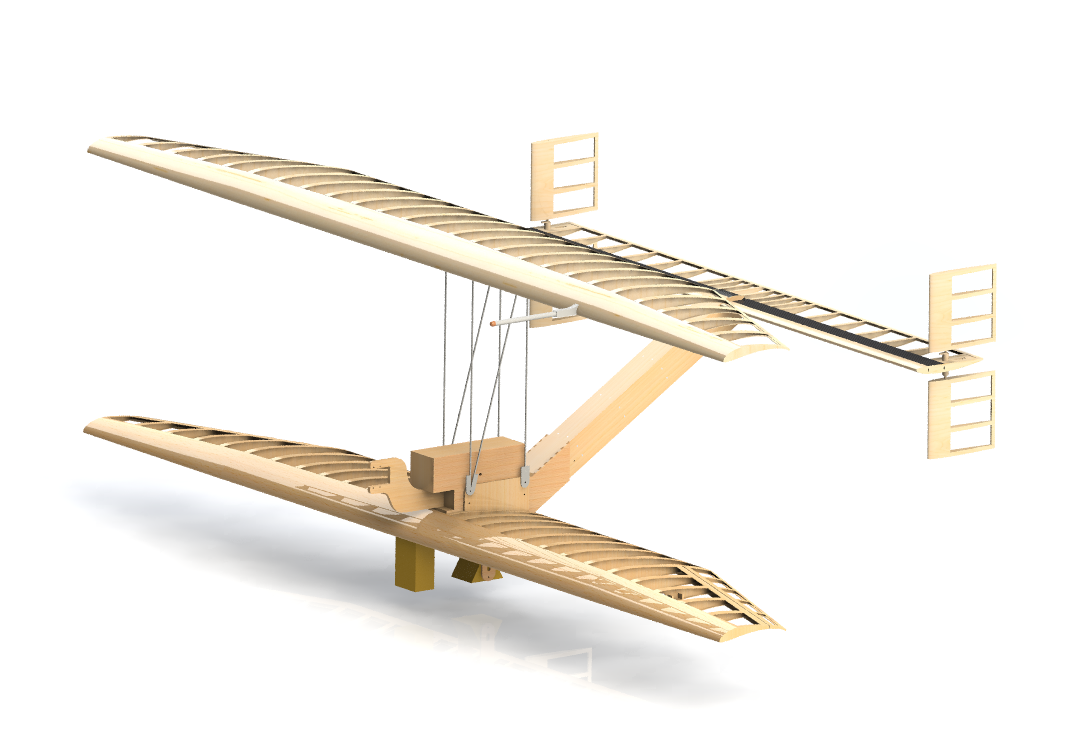
\includegraphics[width=.6\linewidth]{figuras/renders/aviao_sozinho.png}
    \caption{Modelagem da aeronave Céu Azul 2019P1, utilizado nos testes deste trabalho. Fonte: O autor.}
    \label{fig:aviao_renderizado}
\end{figure}

\begin{figure}[!ht]
    \centering
    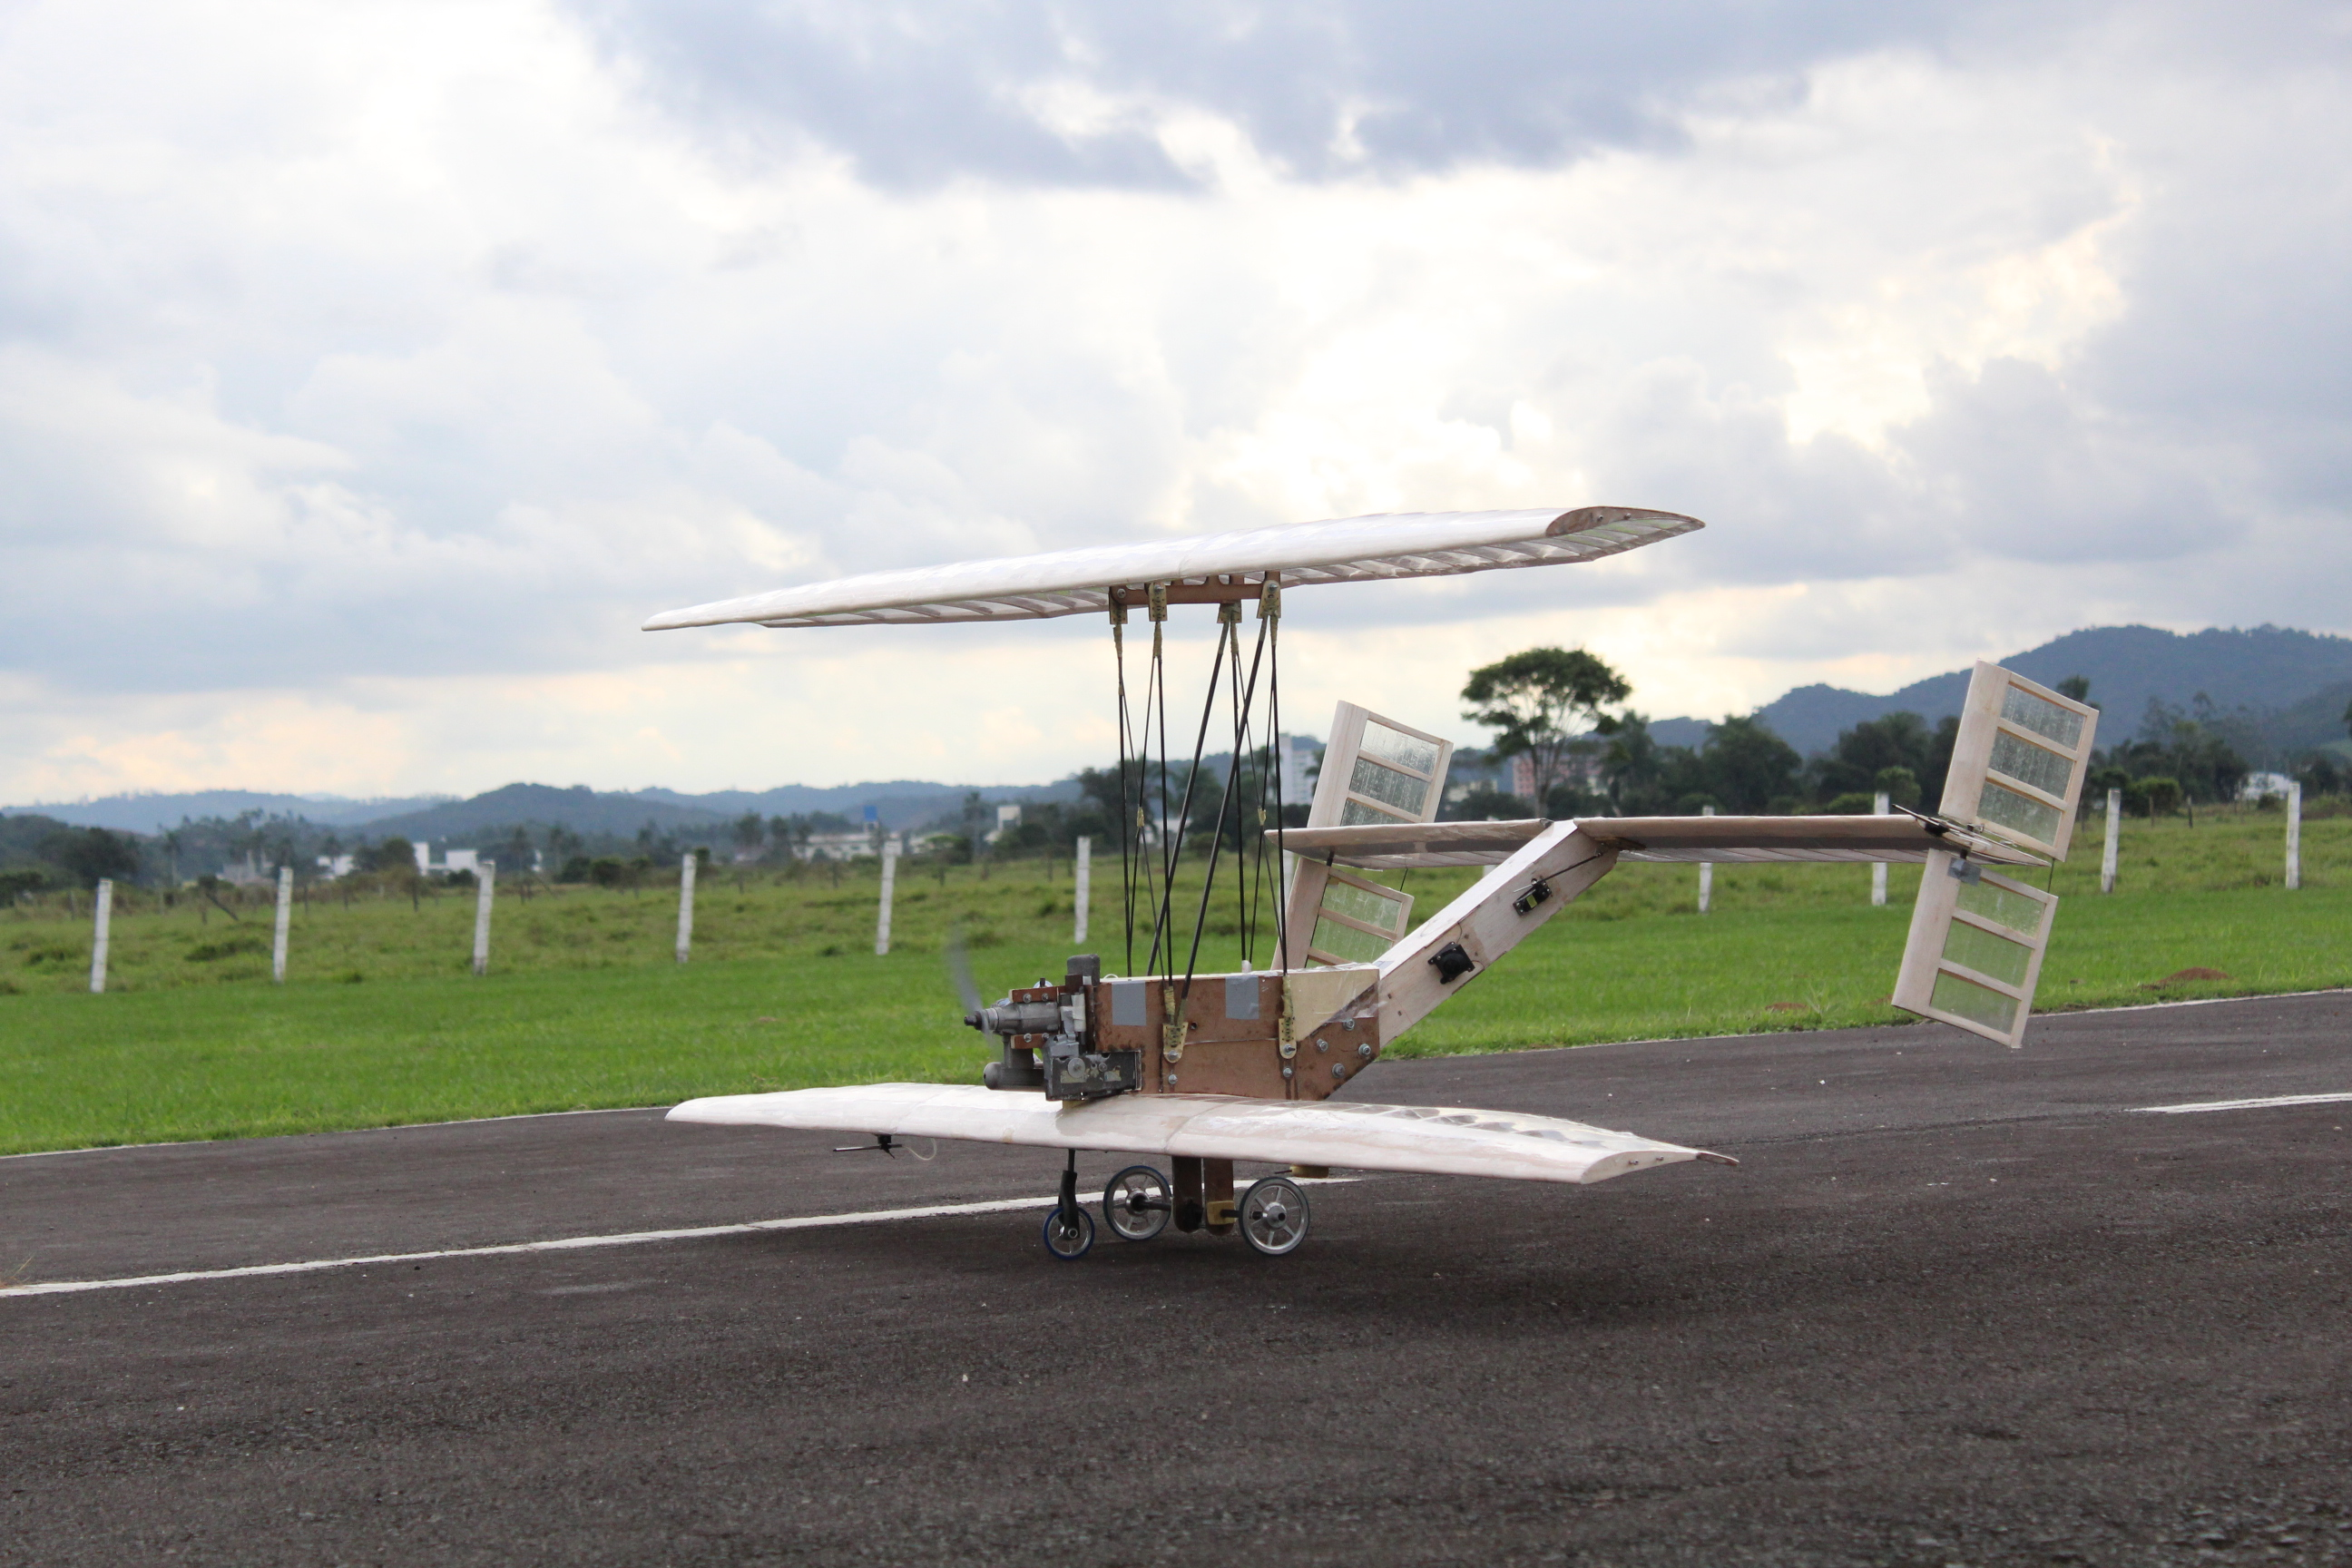
\includegraphics[width=.6\linewidth]{figuras/testes/prototipo_construido.JPG}
    \caption{Foto da aeronave Céu Azul 2019P1, utilizado nos testes deste trabalho. Fonte: O autor.}
    \label{fig:aviao_construido}
\end{figure}

Para a simulação de tal aeronave foi utilizado código de analise ADR, desenvolvido pela equipe Céu Azul Aeronaves com coordenação dO autor.. Este código utiliza para analise aerodinâmica o software de código-aberto AVL, que implementa o algoritmo Vortex Lattice Method, e faz correções de arrasto parasita para cada componente em separado. As figuras \ref{fig:adr_resultados_1} e \ref{fig:adr_resultados_2} mostra as curvas aerodinâmicas simuladas para tal aeronave.

% A figura \ref{fig:avl_simulacao} mostra a simulação de uma das asas da aeronave de teste no software AVL.

% \begin{figure}[!ht]
%     \centering
%     
\includegraphics[width=.8\linewidth]{figuras/outras/placeholder.png}
%     \caption{RENDERING DA SIMULACAO NO AVL. Fonte: O autor.}
%     \label{fig:avl_simulacao}
% \end{figure}

\begin{figure}[!ht]
    \centering
    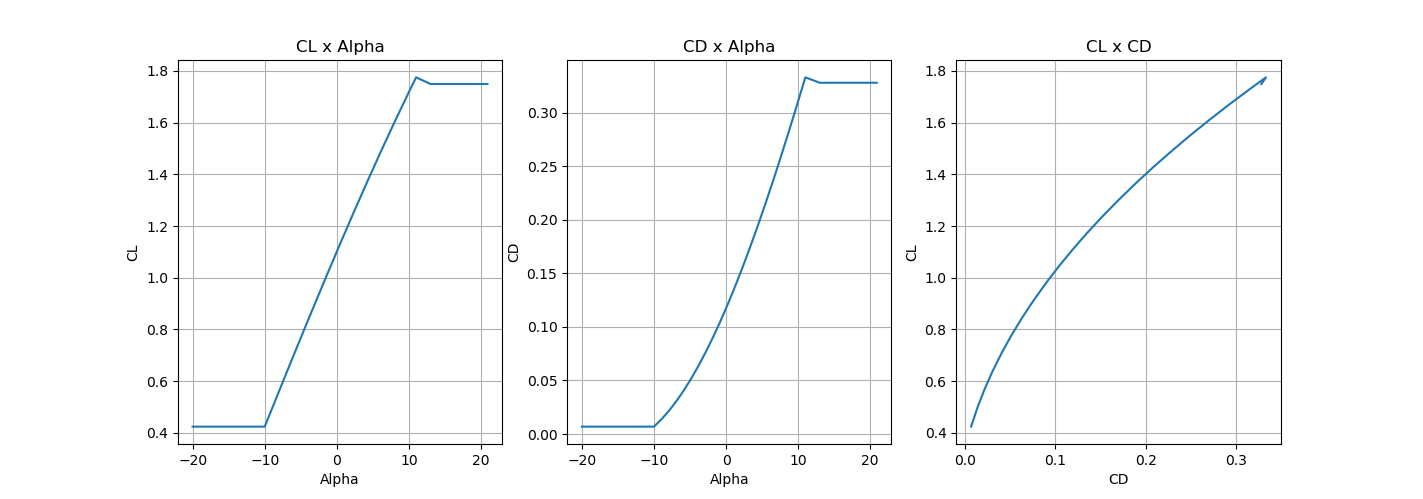
\includegraphics[width=.8\linewidth]{figuras/ADR/cl_cd_polar.png}
    \caption{Graficos de $C_L \times \alpha$, $C_D \times \alpha$ e Polar de Arrasto para a aeronave testada. Fonte: O autor.}
    \label{fig:adr_resultados_1}
\end{figure}

\begin{figure}[!ht]
    \centering
    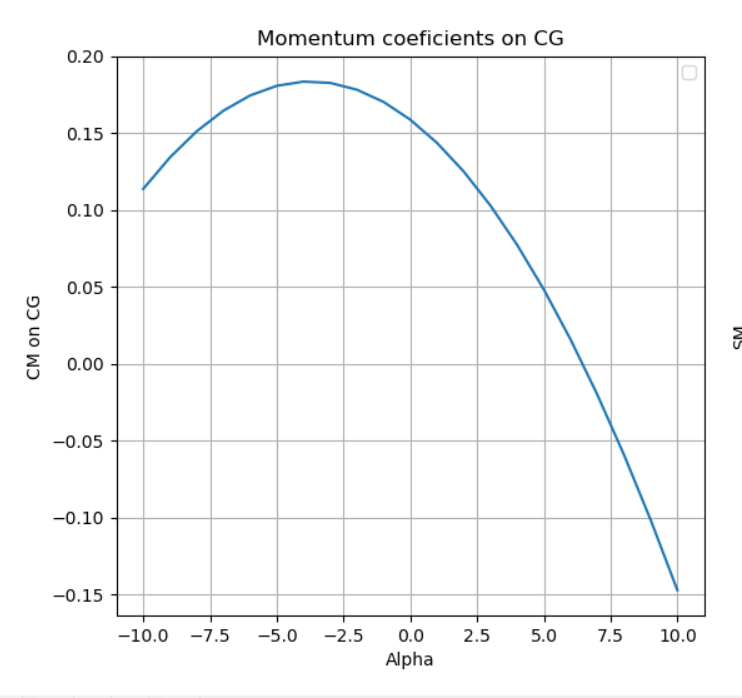
\includegraphics[width=.8\linewidth]{figuras/ADR/cm_alpha_0.png}
    \caption{Gráfico de $C_M \times \alpha$ para a aeronave testada, considerando profundor com 0 graus de ângulo de incidência, como utilizado no teste. Fonte: O autor.}
    \label{fig:adr_resultados_2}
\end{figure}

\subsection{O teste}

Os testes foram conduzidos em uma avenida reta e comprida (Avenida Beira-mar Norte), essencialmente plana e em horário de trânsito reduzido (durante a madrugada).

\begin{figure}[!ht]
    \centering
    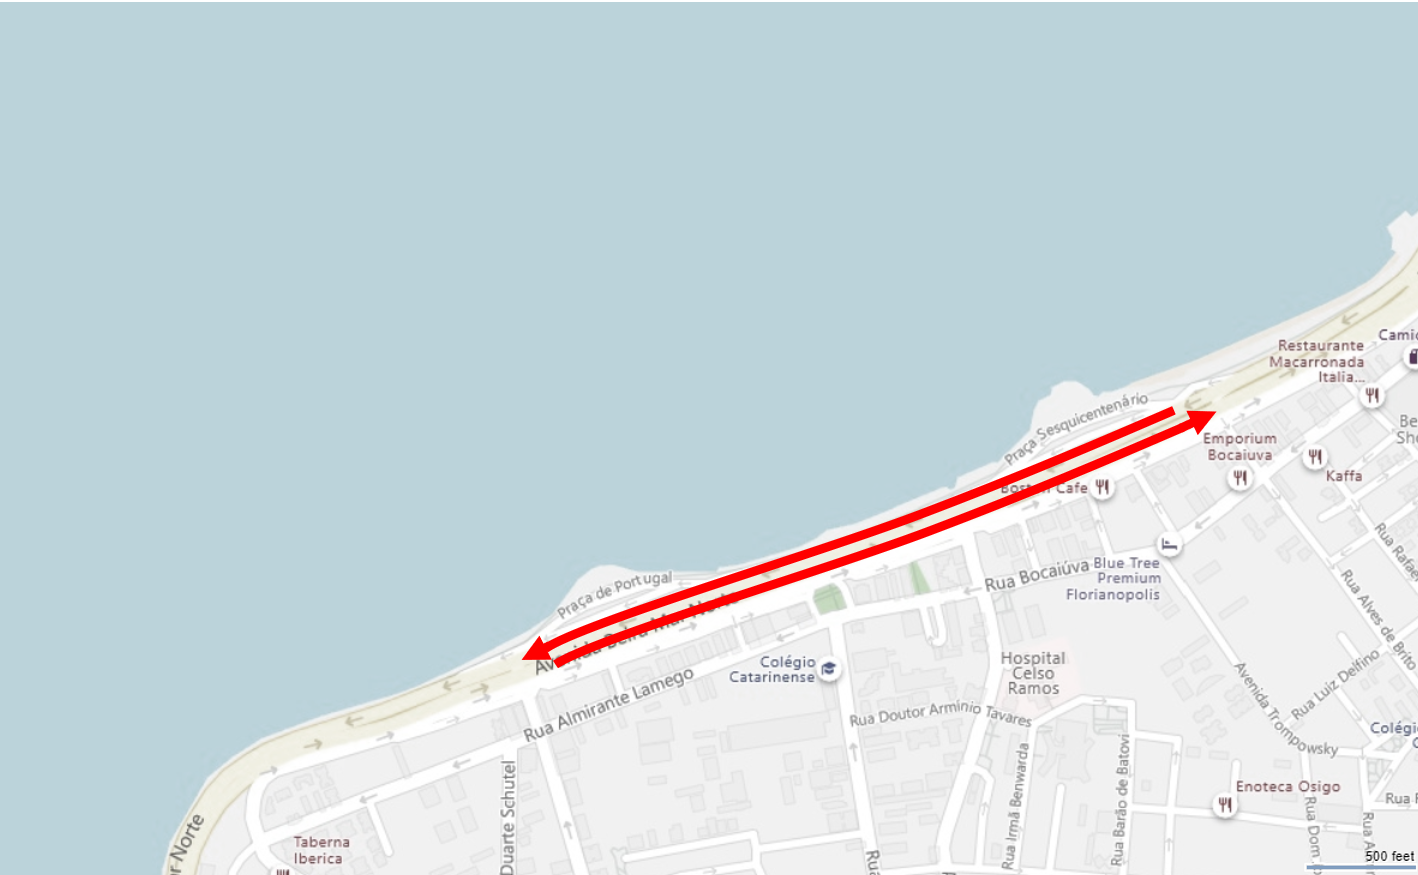
\includegraphics[width=.5\linewidth]{figuras/internet/here_open_street_maps_setas.png}
    \caption{Local onde foram realizados os testes. Fonte: O autor.}
    \label{fig:mapa_teste}
\end{figure}

O teste foi conduzido acelerando-se o carro até uma velocidade de aproximadamente 12m/s (43km/h) e mantendo essa velocidade durante o maior tempo possível. Sendo conduzido desta maneira o teste entrega resultados para apenas um valor de Reynolds. Foi assim feito pois em testes preliminares verificou-se que cada bateria de testes demorava um tempo considerável, e repetir ela para uma grande faixa de Reynolds reduziria o número de dados para cada velocidade. Decidiu-se portanto ter um maior numero de dados para um mesmo Reynolds, garantindo-se uma qualidade melhor dos resultados finais. Com mais tempo porem, ou uma condução mais rápida dos testes, poder-se-ia realizar os testes para mais valores de Reynolds.  

\begin{figure}[!ht]
    \centering
    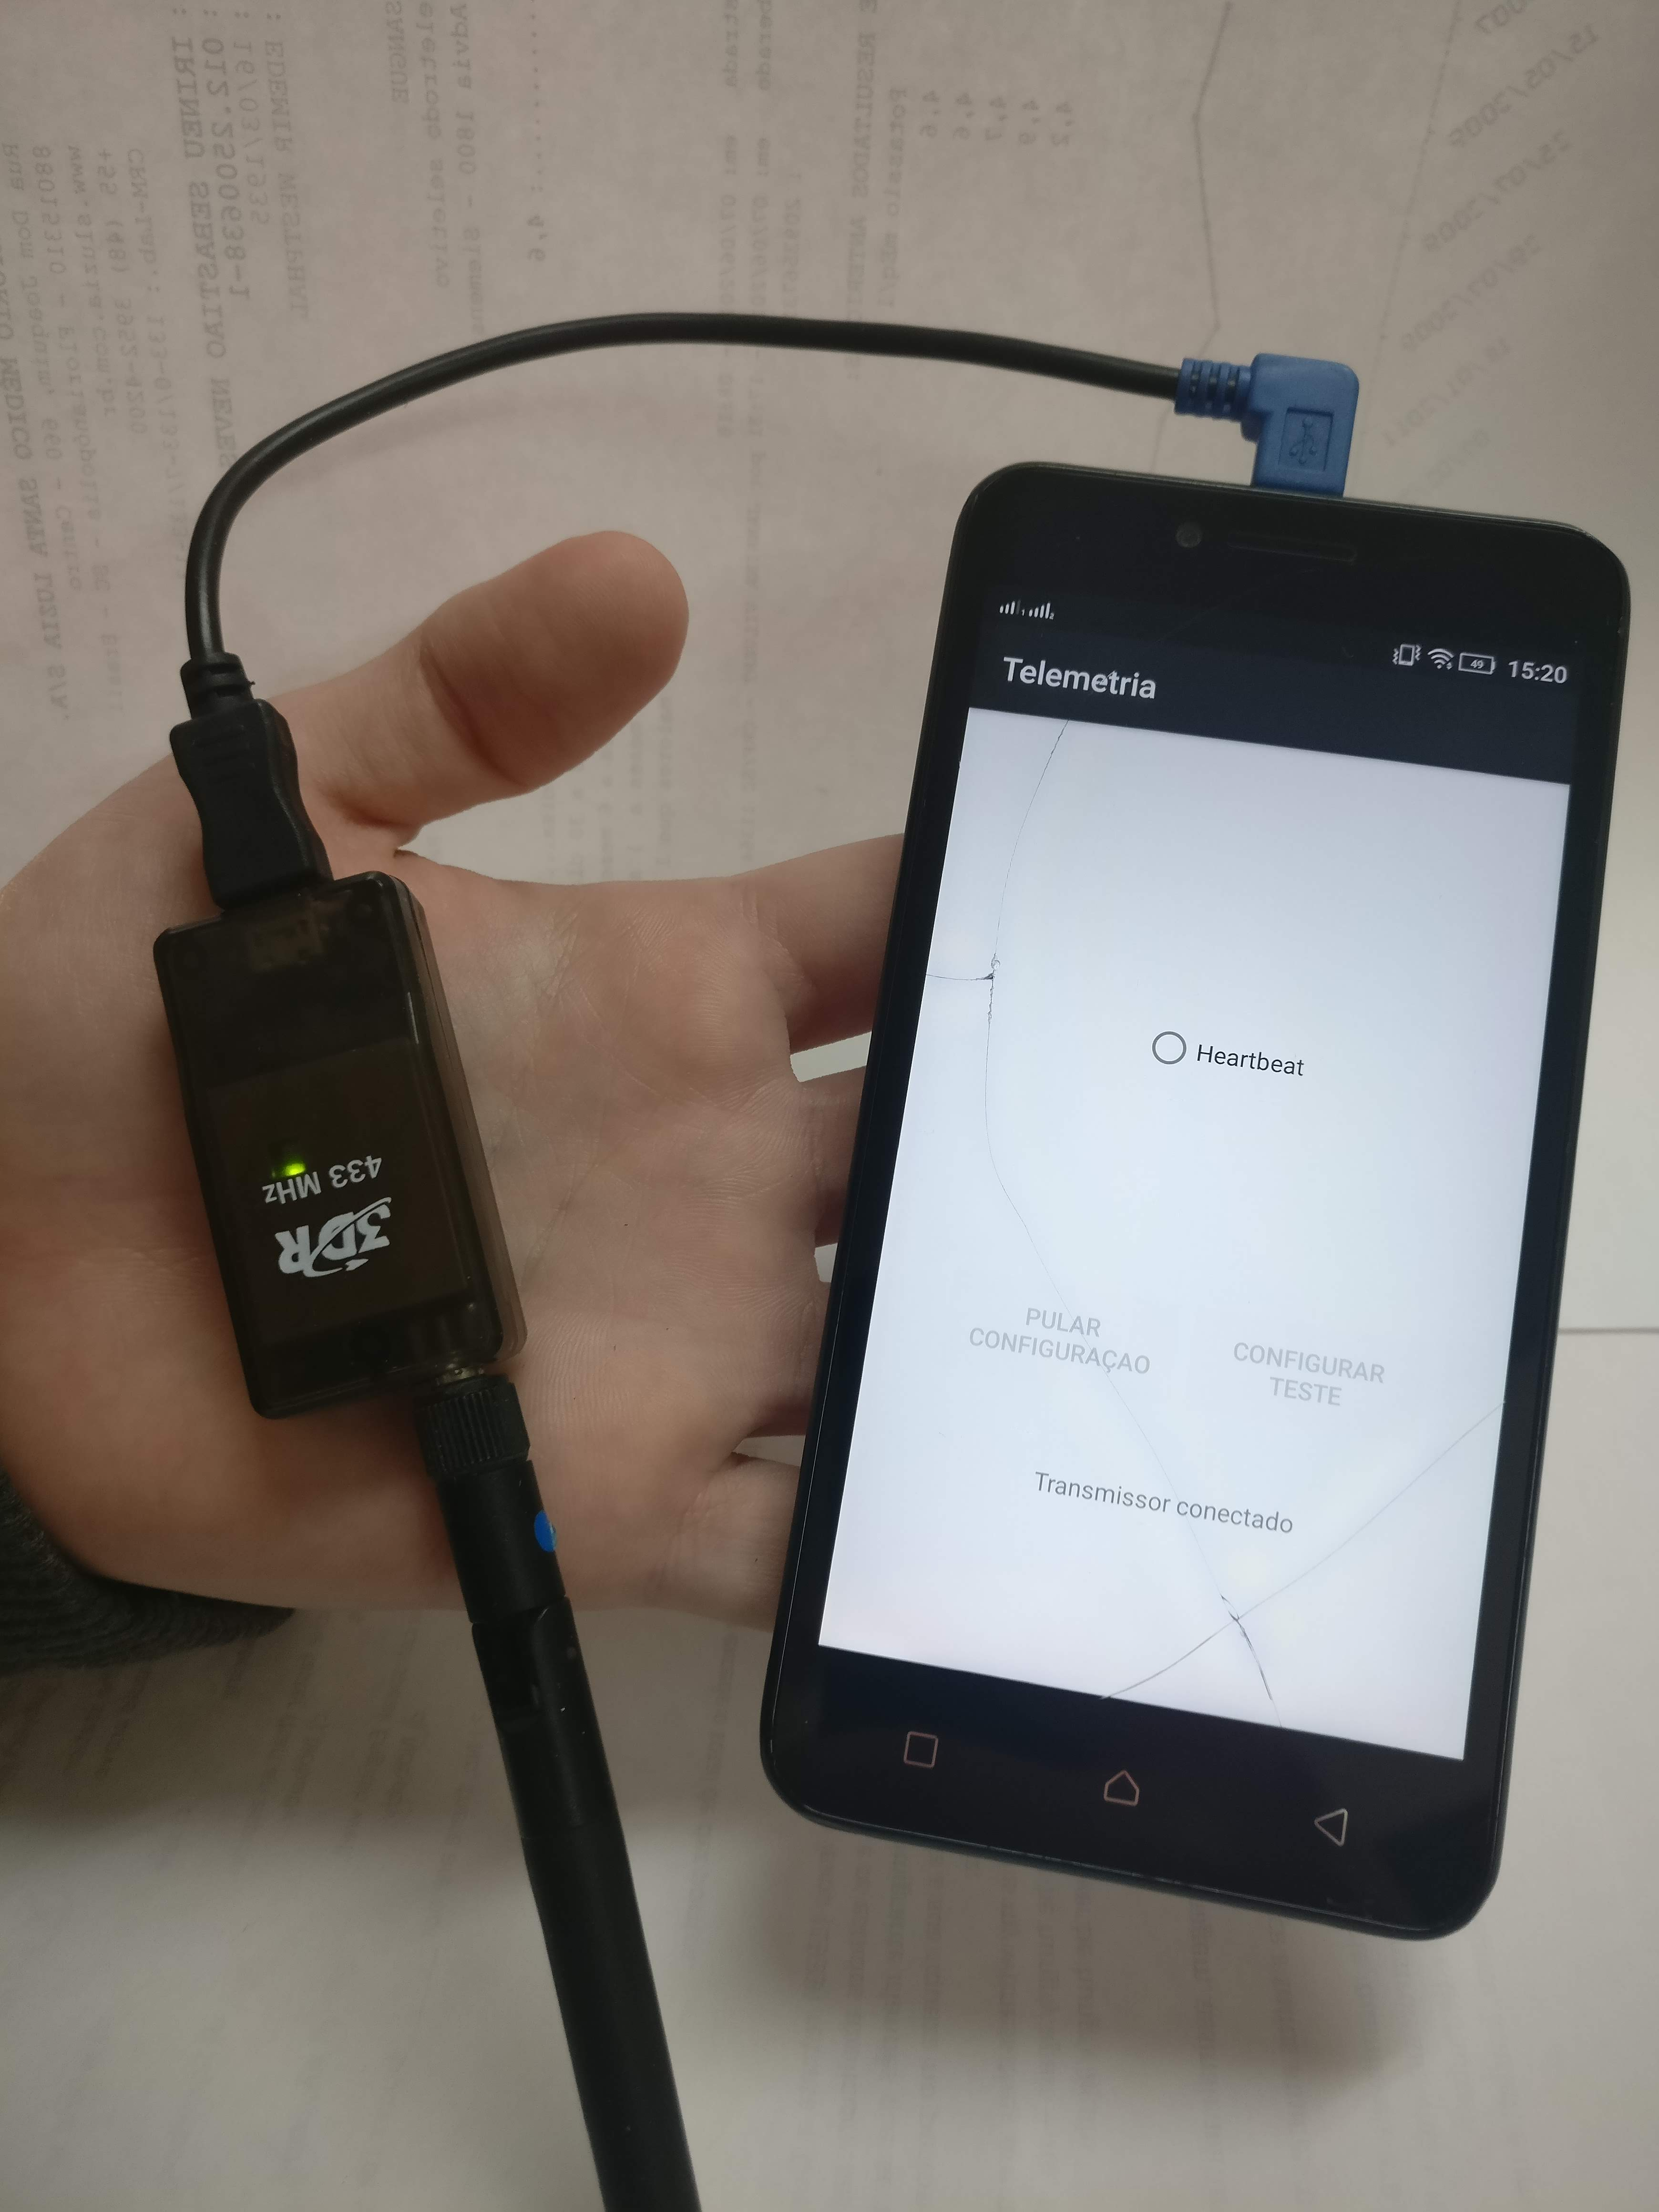
\includegraphics[width=.5\linewidth]{figuras/calibracao/app_celular.jpg}
    \caption{Aplicativo desenvolvido rodando em celular Android com transmissor de radio conectado. Fonte: O autor.}
    \label{fig:app_celular}
\end{figure}

Para se averiguar a velocidade foram utilizados dois recursos: velocímetro do próprio carro e velocidade medida pelo pelos tubos de Pitot. Idealmente as duas medidas devem apresentar o mesmo resultado. Para se acompanhar a velocidade medida pelos Pitots em tempo real foi utilizado o aplicativo desenvolvido.

\begin{figure}[!ht]
    \centering
    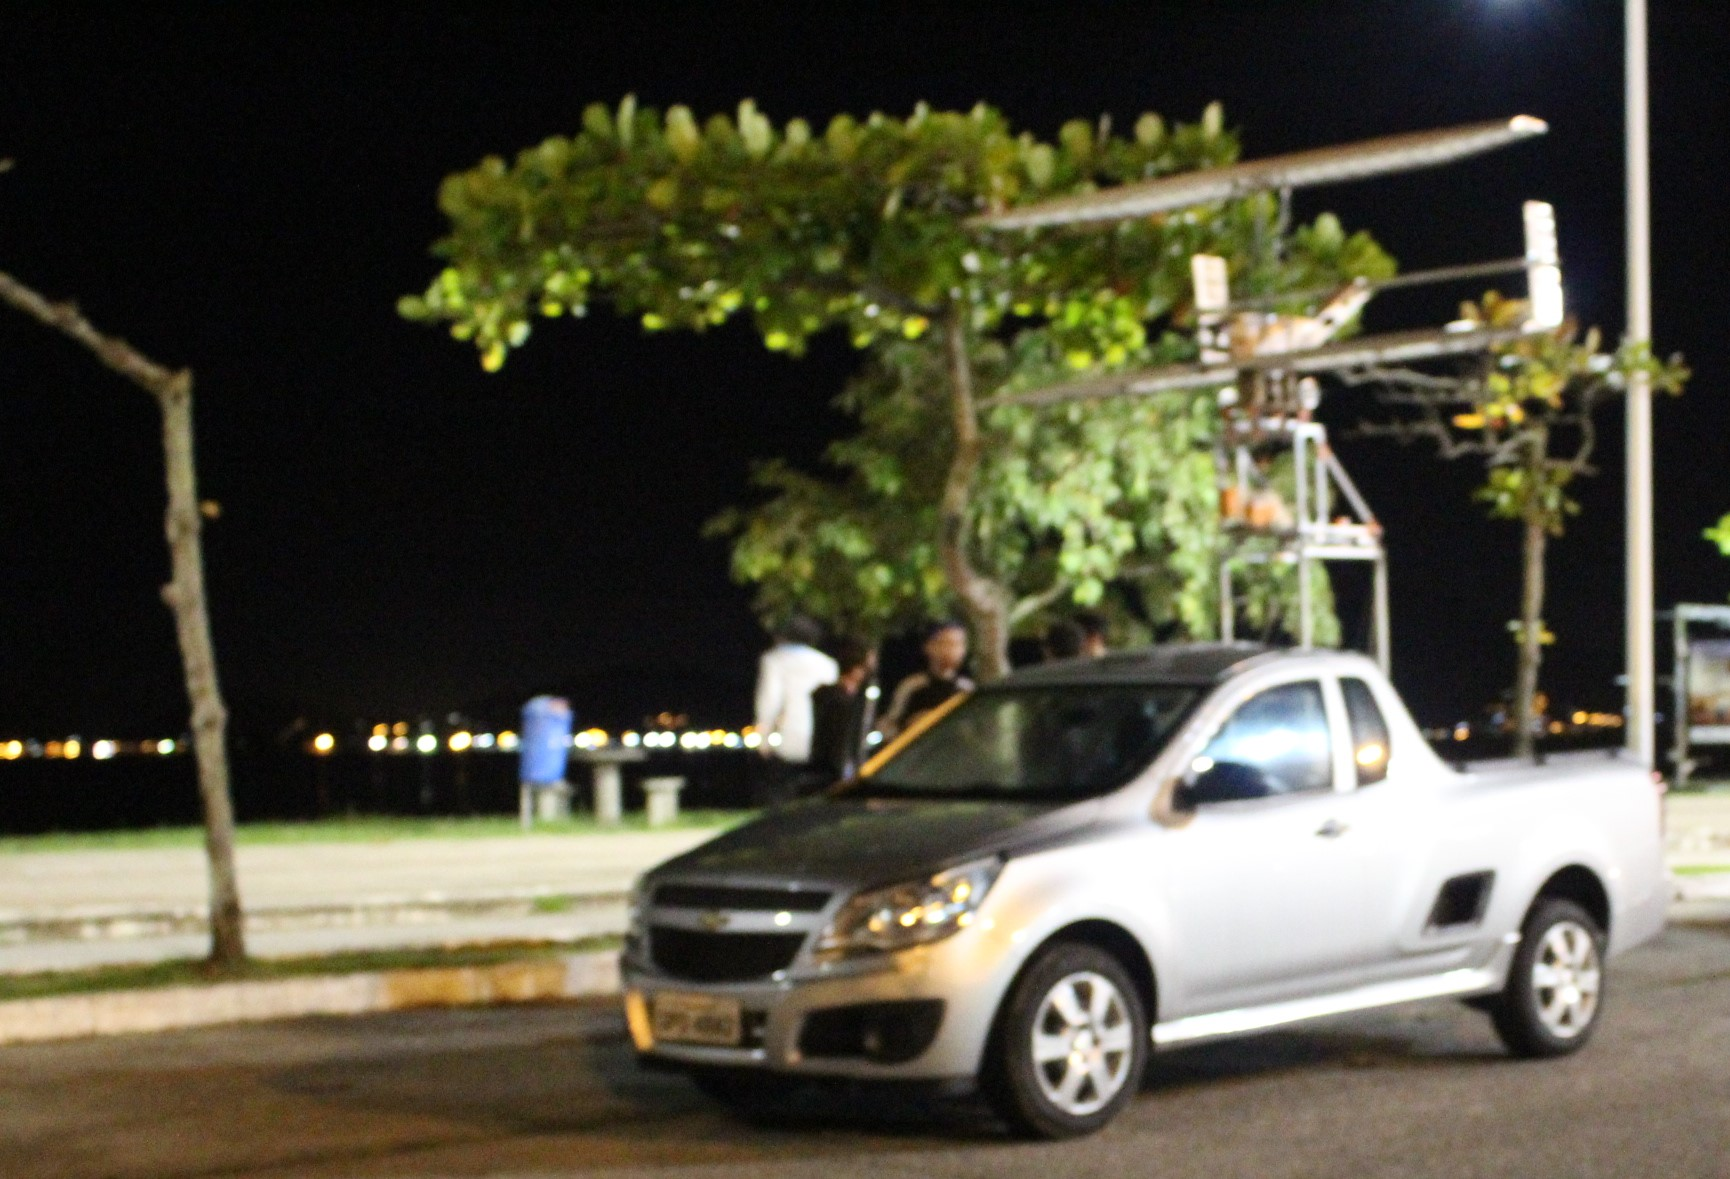
\includegraphics[width=.5\linewidth]{figuras/testes/teste_aviao_completo.JPG}
    \caption{Foto do teste com aeronave Céu Azul 2019 P1. Fonte: O autor.}
    \label{fig:foto_teste_aviao}
\end{figure}

Para cada bateria de testes a asa foi instalada em um ângulo de incidência diferente. Devido a dificuldades técnicas, foram realizados testes apenas para os ângulos de 0, 3 e 6 graus. Para cada um dos ângulos, três baterias de teste foram conduzidas, buscando-se criar uma base de dados grande e diminuir a influencia dos testes nos resultados.

